
\chapter{Continuous pressure measurement}

In many ways, pressure is the primary variable for a wide range of process measurements.  Many types of industrial measurements are actually inferred from pressure, such as:  \index{Inferred variable}

\begin{itemize}
\item Flow (measuring the pressure dropped across a restriction)
\item Liquid level (measuring the pressure created by a vertical liquid column)
\item Liquid density (measuring the pressure difference across a fixed-height liquid column)
\item Weight (hydraulic load cell)
\end{itemize}

Even temperature may be inferred from pressure measurement, as in the case of a fluid-filled chamber where fluid pressure and fluid temperature are directly related.  As such, pressure is a very important quantity to measure, and measure accurately.  This section describes different technologies for the measurement of pressure.  \index{Inferred variable}






\filbreak
\section{Manometers}

A very simple device used to measure pressure is the \textit{manometer}: a fluid-filled tube where an applied gas pressure causes the fluid height to shift proportionately.  This is why pressure is often measured in units of liquid height (e.g. inches of water, inches of mercury).  As you can see, a manometer is fundamentally an instrument of \textit{differential} pressure measurement, indicating the difference between two pressures by a shift in liquid column height: \index{Manometer}

$$\includegraphics{005.eps}$$

Of course, it is entirely acceptable to simply vent one tube of a manometer and use it as a \textit{gauge} pressure instrument, comparing the applied pressure at one tube against atmospheric pressure in the other.

\filbreak

Liquid column height in a manometer should always be interpreted at the centerline of the liquid column, regardless of the shape of the liquid's meniscus (the curved air/liquid interface): \index{Meniscus}

$$\includegraphics{006.eps}$$

\filbreak

Manometers come in a variety of forms, the most common being the \textit{U-tube}, \textit{well} (sometimes called a \textit{cistern}), \textit{raised well}, and \textit{inclined}: \index{Manometer, U-tube} \index{Manometer, well} \index{Manometer, raised well} \index{Manometer, inclined} \index{Inclined manometer} \index{U-tube manometer} \index{Well manometer}  \index{Raised well manometer}  \index{Cistern manometer} \index{Manometer, cistern}

$$\includegraphics{007.eps}$$

$$\includegraphics{008.eps}$$

\filbreak

U-tube manometers are very inexpensive, and are generally made from clear plastic (see the left-hand photo).  Cistern-style manometers are the norm for calibration bench work, and are typically constructed from metal cisterns and glass tubes (see the right-hand photo):

$$\includegraphics[width=2in]{u_tube_manometer.eps} \hskip 30pt \includegraphics[width=2in]{cistern_manometers.eps}$$

\filbreak

Inclined manometers are used to measure very low pressures, owing to their exceptional sensitivity (note the fractional scale for inches of water column in the following photograph, extending from 0 to 1.5 inches on the scale, reading left to right):

$$\includegraphics[width=5in]{inclined_manometer.eps}$$

Note that venting one side of a manometer is standard practice when using it as a \textit{gauge pressure} indicator (responding to pressure in excess of atmospheric).  Both pressure ports will be used if the manometer is applied to the measurement of differential pressure, just as in the case of the U-tube manometer first shown in this section.  Absolute pressure may also be measured by a manometer, if one of the pressure ports connects to a sealed vacuum chamber.  This is how a \textit{mercury barometer} is constructed for the measurement of absolute ambient air pressure: by sealing off one side of a manometer and removing all the air in that side, such that the applied (atmospheric) pressure is always compared against a vacuum. \index{Barometer} \index{Mercury barometer} \index{Absolute pressure} \index{Differential pressure} \index{Gauge pressure}

Manometers incorporating a ``well'' have the advantage of single-point reading: one need only compare the height of \textit{one} liquid column, not the difference in height between \textit{two} liquid columns.  The cross-sectional area of the liquid column in the well is so much greater than that within the transparent manometer tube that the change in height within the well is usually negligible.  In cases where the difference is significant, the spacing between divisions on the manometer scale may be skewed to compensate\footnote{If you are having difficulty understanding this concept, imagine a simple U-tube manometer where one of the tubes is opaque, and therefore one of the two liquid columns cannot be seen.  In order to be able to measure pressure just by looking at one liquid column height, we would have to make a custom scale where every inch of height registered as \textit{two} inches of water column pressure, because for each inch of height change in the liquid column we can see, the liquid column we can't see also changes by an inch.  A scale custom-made for a well-type manometer is just the same concept, only without such dramatic skewing of scales.}.

Inclined manometers enjoy the advantage of increased sensitivity.  Since manometers fundamentally operate on the principle of pressure balanced by liquid height, and this liquid height is always measured parallel to the line of gravitational pull (perfectly vertical), inclining the manometer tube means that liquid must travel farther along the tube to generate the same change in (purely) vertical height than it would in a vertical manometer tube.  Thus, an inclined manometer tube causes an amplification in liquid motion for a given amount of pressure change, allowing measurements of greater resolution.





\filbreak
\section{Mechanical pressure elements}

Mechanical pressure-sensing elements include the \textit{bellows}, the \textit{diaphragm}, and the \textit{bourdon tube}.  Each of these devices converts a fluid pressure into a force.  If unrestrained, the natural elastic properties of the element will produce a motion proportional to the applied pressure.  \index{Bellows} \index{Diaphragm} \index{Bourdon tube}

$$\includegraphics{003.eps}$$

Bellows resemble an accordion constructed from metal instead of fabric.  Increasing pressure inside a bellows unit causes it to elongate.  A photograph of a bellows is shown here:

$$\includegraphics[width=4in]{pneumatics35.eps}$$

A diaphragm is nothing more than a thin disk of material which bows outward under the influence of a fluid pressure.  Many diaphragms are constructed from metal, which gives them spring-like qualities.  Some diaphragms are intentionally constructed out of materials with little strength, such that there is negligible spring effect.  These are called \textit{slack diaphragms}, and they are used in conjunction with external mechanisms (e.g. springs) producing the necessary restraining force to prevent damage from applied pressure.  \index{Slack diaphragm} 

\filbreak

The following photograph shows the mechanism of a small pressure gauge using a brass diaphragm as the sensing element:

$$\includegraphics[width=5in]{gauge_diaphragm.eps}$$

As pressure is applied to the rear of the diaphragm, it distends upward (away from the table on which it rests as shown in the photograph), causing a small shaft to twist in response.  This twisting motion is transferred to a lever which pulls on a tiny link chain wrapped around the pointer shaft, causing it to rotate and move the pointer needle around the gauge scale.  Both the needle and scale on this gauge mechanism have been removed for easier viewing of diaphragm and mechanism.

\vskip 10pt

Bourdon tubes are made of spring-like metal alloys bent into a circular shape.  Under the influence of internal pressure, a bourdon tube ``tries'' to straighten out into its original shape before being bent at the time of manufacture.

Most pressure gauges use a bourdon tube as their pressure-sensing element.  Most pressure transmitters use a diaphragm as their pressure-sensing element.  Bourdon tubes may be made in \textit{spiral} or \textit{helical} forms for greater motion (and therefore greater gauge resolution).  \index{Helical bourdon tube} \index{Spiral bourdon tube}

\filbreak

The Bourdon tube pressure element is a very robust and time-tested design.  An illustration taken from page 471 of volume 1 of \textit{Cassier's Magazine} published in the year 1891 shows a typical C-shaped bourdon tube pressure gauge mechanism complete with gears and pointing needle:  \index{Pressure gauge mechanism, typical}  \index{Bourdon tube}

$$\includegraphics[height=6in]{020.eps}$$

Looking closely at the labeled components of this mechanism, we see a circular ``pinion'' touching a curved ``sector''.  Both of these are \textit{gears} meshing with one another, but as is typical with mechanical drawings the individual teeth of the meshing gears are not shown.

It is a useful mental exercise to imagine the components of this gauge moving under the influence of a rising fluid pressure.  The bourdon tube will straighten, resulting in its tip extending outward from center (up and right) as its socket remains stationary (anchored to the gauge body).  This pulls on the link, which in turn causes the sector gear to rotate counter-clockwise on its bearing axis (that axis anchored on the backing plate of the gauge).  This causes the pinion gear to rotate clockwise, driving the needle (the ``indexing hand'') clockwise as well, so that the needle's tip rises up the numerical scale printed on the gauge face.

\filbreak

A photograph of a C-tube pressure gauge mechanism (taken from the rear of the gauge, behind the pointer and scale) reveals its mechanical workings:

$$\includegraphics[width=3in]{bourdon_tube_closeup.eps}$$

The dark, C-shaped tube is the bourdon tube sensing element, while the shiny metal parts are the linkage, lever, and gear assembly.

\filbreak

The next photograph shows a \textit{spiral} bourdon tube, designed to produce a wider range of motion than a C-tube bourdon:

$$\includegraphics[width=4in]{spiral_bourdon.eps}$$

\vskip 10pt

It should be noted that bellows, diaphragms, and bourdon tubes alike may all be used to measure differential and/or absolute pressure in addition to gauge pressure.  All that is needed for these other functionalities is to subject the \textit{other} side of each pressure-sensing element to either another applied pressure (in the case of differential measurement) or to a vacuum chamber (in the case of absolute pressure measurement).

\filbreak

This next set of illustrations shows how bellows, diaphragms, and bourdon tubes may be used as differential pressure-sensing elements:

$$\includegraphics{019.eps}$$

The challenge in doing this, of course, is how to extract the mechanical motion of the pressure-sensing element to an external mechanism (such as a pointer) while maintaining a good pressure seal.  In gauge pressure mechanisms, this is no problem because one side of the pressure-sensing element must be exposed to atmospheric pressure anyway, and so that side is always available for mechanical connection.

A differential pressure gauge is shown in the next photograph.  The two pressure ports are clearly evident on either side of the gauge:

$$\includegraphics[width=3in]{pressure53.eps}$$




\filbreak
\section{Electrical pressure elements}

Several different technologies exist for the conversion of fluid pressure into an electrical signal response.  These technologies form the basis of electronic \textit{pressure transmitters}: devices designed to measure fluid pressure and transmit that information via electrical signals such as the 4-20 mA analog standard, or in digital form such as HART or FOUNDATION Fieldbus.

A brief survey of electronic pressure transmitters in contemporary\footnote{As of this writing, 2008.} use reveals a diverse representation of electrical pressure-sensing elements:

% No blank lines allowed between lines of an \halign structure!
% I use comments (%) instead, so Tex doesn't choke.

$$\vbox{\offinterlineskip
\halign{\strut
\vrule \quad\hfil # \ \hfil & 
\vrule \quad\hfil # \ \hfil & 
\vrule \quad\hfil # \ \hfil \vrule \cr
\noalign{\hrule}
%
% First row
\textbf{Manufacturer} & \textbf{Model} & \textbf{Pressure sensor technology} \cr
%
\noalign{\hrule}
%
% Another row
%ABB/Bailey & 2600T & Differential reluctance (?) \cr
%
%\noalign{\hrule}
%
% Another row
ABB/Bailey & PTSD & Differential reluctance \cr
%
\noalign{\hrule}
%
% Another row
ABB/Bailey & PTSP & Piezoresistive (strain gauge) \cr
%
\noalign{\hrule}
%
% Another row
Foxboro & IDP10 & Piezoresistive (strain gauge) \cr
%
\noalign{\hrule}
%
% Another row
Honeywell & ST3000 & Piezoresistive (strain gauge) \cr
%
\noalign{\hrule}
%
% Another row
Rosemount & 1151 & Differential capacitance \cr
%
\noalign{\hrule}
%
% Another row
Rosemount & 3051 & Differential capacitance \cr
%
\noalign{\hrule}
%
% Another row
Rosemount & 3095 & Differential capacitance \cr
%
\noalign{\hrule}
%
% Another row
Yokogawa & EJX series & Mechanical resonance \cr
%
\noalign{\hrule}
} % End of \halign 
}$$ % End of \vbox








\filbreak
\subsection{Piezoresistive (strain gauge) sensors}

\textit{Piezoresistive} means ``pressure-sensitive resistance,'' or a resistance that changes value with applied pressure.  The \textit{strain gauge} is a classic example of a piezoresistive element, a typical strain gauge element shown here on the tip of my finger:  \index{Strain gauge}

$$\includegraphics[width=4in]{bridge08.eps}$$

In order to be practical, a strain gauge must be glued (\textit{bonded}) on to a larger specimen capable of withstanding an applied force (stress):

$$\includegraphics{bridge05.eps}$$

As the test specimen is stretched or compressed by the application of force, the conductors of the strain gauge are similarly deformed.  Electrical resistance of any conductor is proportional to the ratio of length over cross-sectional area ($R \propto {l \over A}$), which means that tensile deformation (stretching) will increase electrical resistance by simultaneously increasing length and decreasing cross-sectional area while compressive deformation (squishing) will decrease electrical resistance by simultaneously decreasing length and increasing cross-sectional area.

Attaching a strain gauge to a diaphragm results in a device that changes resistance with applied pressure.  Pressure forces the diaphragm to deform, which in turn causes the strain gauge to change resistance.  By measuring this change in resistance, we can infer the amount of pressure applied to the diaphragm.

The classic strain gauge system represented in the previous illustration is made of metal (both the test specimen and the strain gauge itself).  Within its elastic limits, many metals exhibit good spring characteristics.  Metals, however, are subject to \textit{fatigue} over repeated cycles of strain (tension and compression), and they will begin to ``flow'' if strained beyond their elastic limit.  This is a common source of error in metallic piezoresistive pressure instruments: if overpressured, they tend to lose accuracy due to damage of the spring and strain gauge elements.\footnote{For a simple demonstration of metal fatigue and metal ``flow,'' simply take a metal paper clip and repeatedly bend it back and forth until you feel the metal wire weaken.  Gentle force applied to the paper clip will cause it to deform in such a way that it returns to its original shape when the force is removed.  Greater force, however, will exceed the paper clip's elastic limit, causing permanent deformation and also altering the spring characteristics of the clip.}  \index{Metal fatigue}

Modern manufacturing techniques have made possible the construction of strain gauges made of silicon instead of metal.  Silicon exhibits very linear spring characteristics over its narrow range of motion, and a high resistance to fatigue.  When a silicon strain gauge is over-stressed, it fails completely rather than ``flows'' as is the case with metal strain gauges.  This is generally considered a better result, as it clearly indicates the need for sensor replacement (whereas a metallic strain sensor may give the false impression of continued function following an over-stress event).  \index{Silicon strain gauge element}

\filbreak

Thus, most modern piezoresistive-based pressure instruments use silicon strain gauge elements to sense deformation of a diaphragm due to applied fluid pressure.  A simplified illustration of a diaphragm / strain gauge pressure sensor is shown here:

$$\includegraphics{pressure49.eps}$$

As the diaphragm bows outward with applied fluid pressure, the strain gauge stretches to a greater length, causing its resistance to increase.  This change in resistance imbalances the bridge circuit, causing a voltage ($V_{out}$) proportional to the amount of applied pressure.  Thus, the strain gauge works to convert an applied pressure into a measurable voltage signal which may be amplified and converted into a 4-20 mA loop current signal (or into a digital ``fieldbus'' signal).

% ADD: show illustrations exaggerating the deformation of the diaphragm, both with an applied pressure and an applied vacuum

\filbreak

In some designs, a single silicon wafer serves as both the diaphragm and the strain gauge so as to fully exploit the excellent mechanical properties of silicon (high linearity and low fatigue).  However, silicon is not chemically compatible with many process fluids, and so pressure must be transferred to the silicon diaphragm/sensor via a non-reactive \textit{fill fluid} (commonly a silicone-based or fluorocarbon-based liquid).  A metal \textit{isolating diaphragm} transfers process fluid pressure to the fill fluid, which in turn transfers pressure to the silicon wafer.  Another simplified illustration shows how this works: \index{Isolating diaphragm} \index{Diaphragm, isolating} \index{Fill fluid}

$$\includegraphics{pressure50.eps}$$

The isolating diaphragm is designed to be much more flexible (less rigid) than the silicon diaphragm, because its purpose is to seamlessly transfer fluid pressure from the process fluid to the fill fluid, not to act as a spring element.  In this way, the silicon sensor experiences the same pressure that it would if it were directly exposed to the process fluid, without having to contact the process fluid.  The flexibility of the metal isolating diaphragm also means it experiences much less stress than the silicon sensing diaphragm, which avoiding the problems of metal fatigue experienced by transmitter designs using metal as the sensing (spring) element.

This use of a fill fluid to transfer pressure from an isolating diaphragm to a sensing diaphragm inside the transmitter is used in most if not all modern pressure transmitter designs, even those that are not piezoresistive.

\filbreak

An example of a pressure instrument utilizing a silicon strain gauge element is the Foxboro model IDP10 differential pressure transmitter, shown in the following photograph:  \index{Foxboro model IDP10 differential pressure transmitter}

$$\includegraphics[width=3in]{dpcell_5.eps}$$






\filbreak
\subsection{Differential capacitance sensors}

Another common electrical pressure sensor design works on the principle of \textit{differential capacitance}.  In this design, the sensing element is a taut metal diaphragm located equidistant between two stationary metal surfaces\footnote{In the following diagram, both the sensing diaphragm and the stationary metal surfaces are shown colored blue, to distinguish these electrical elements from the other structural components of the device.}, comprising three plates for a complementary pair of capacitors.  An electrically insulating fill fluid (usually a liquid silicone compound) transfers motion from the isolating diaphragms to the sensing diaphragm, and also doubles as an effective dielectric for the two capacitors: \index{Differential capacitance pressure sensor} \index{Isolating diaphragm} \index{Diaphragm, isolating} \index{Fill fluid}

$$\includegraphics{pressure31.eps}$$

Any difference of pressure across the cell causes the diaphragm to flex in the direction of least pressure.  The sensing diaphragm is a precision-manufactured spring element, meaning that its displacement is a predictable function of applied force.  The applied force in this case can only be a function of differential pressure acting against the surface area of the diaphragm in accordance with the standard force-pressure-area equation $F=PA$.  In this case, we have two forces caused by two fluid pressures working against each other, so our force-pressure-area equation may be re-written to describe \textit{resultant} force as a function of differential pressure ($P_1 - P_2$) and diaphragm area: $F = (P_1 - P_2)A$.  Since diaphragm area is constant, and force is predictably related to diaphragm displacement, all we need now in order to infer differential pressure is to accurately measure displacement of the diaphragm.

\filbreak

The diaphragm's secondary function as one plate of two capacitors provides a convenient method for measuring displacement.  Since capacitance between conductors is inversely proportional to the distance separating them, capacitance on the low-pressure side will increase while capacitance on the high-pressure side will decrease:

$$\includegraphics{pressure32.eps}$$

A capacitance detector circuit connected to this cell uses a high-frequency AC excitation signal to measure the different in capacitance between the two halves, translating that into a DC signal which ultimately becomes the signal output by the instrument representing pressure.

These pressure sensors are highly accurate, stable, and rugged.  An interesting feature of this design -- using two isolating diaphragms to transfer process fluid pressure to a single sensing diaphragm through an internal ``fill fluid'' -- is that the solid frame bounds the motion of the two isolating diaphragms such that neither one is able to force the sensing diaphragm past its elastic limit.  As the illustration shows, the higher-pressure isolating diaphragm gets pushed toward the metal frame, transferring its motion to the sensing diaphragm via the fill fluid.  If too much pressure is applied to that side, the isolating diaphragm will merely ``flatten'' against the solid frame of the capsule and stop moving.  This positively limits the isolating diaphragm's motion so that it cannot possibly exert any more force on the sensing diaphragm, even if additional process fluid pressure is applied.  This use of isolating diaphragms and fill fluid to transfer motion to the sensing diaphragm, employed in other styles of differential pressure sensor as well, gives modern differential pressure instruments excellent resistance to overpressure damage.

It should be noted that the use of a liquid fill fluid is key to this overpressure-resistant design.  In order for the sensing diaphragm to accurately translate applied pressure into a proportional capacitance, it must not contact the conductive metal frame surrounding it.  In order for any diaphragm to be protected against overpressure, however, it must contact a solid backstop to limit further travel.  Thus, the need for non-contact (capacitance) and for contact (overpressure protection) are mutually exclusive, making it nearly impossible to perform both functions with a single sensing diaphragm.  Using fill fluid to transfer pressure from isolating diaphragms to the sensing diaphragm allows us to separate the function of capacitive measurement (sensing diaphragm) from the function of overpressure protection (isolation diaphragms) so that each diaphragm may be optimized for a separate purpose.  \index{Fill fluid}

\filbreak

A classic example of a pressure instrument based on the differential capacitance sensor is the Rosemount model 1151 differential pressure transmitter, shown in assembled form in the following photograph: \index{Rosemount model 1151 differential pressure transmitter}

$$\includegraphics[width=5in]{diff_capacitance_1.eps}$$

\filbreak

By removing four bolts from the transmitter, we are able to remove two flanges from the pressure capsule, exposing the isolating diaphragms to plain view:

$$\includegraphics[width=5in]{diff_capacitance_3.eps}$$

A close-up photograph shows the construction of one of the isolating diaphragms, which unlike the sensing diaphragm is designed to be very flexible.  The concentric corrugations in the metal of the diaphragm allow it to easily flex with applied pressure, transmitting process fluid pressure through the silicone fill fluid to the taut sensing diaphragm inside the differential capacitance cell: \index{Isolating diaphragm} \index{Diaphragm, isolating} \index{Fill fluid}

$$\includegraphics[width=4in]{diff_capacitance_4.eps}$$

\filbreak

The interior of the same differential capacitance sensor (revealed by cutting a Rosemount model 1151 sensor in half with a chop saw\footnote{A chop saw is admittedly not a tool of finesse, and it did a fair job of mangling this unfortunate differential capacitance cell.  A bandsaw was tried at first, but made virtually no progress in cutting the hard stainless steel of the capsule assembly.  The chop saw's abrasive wheel created a lot of heat, discoloring the metal and turning the silicone fill fluid into a crystalline mass which had to be carefully chipped out by hand using an ice pick so as to not damage the thin metal sensing diaphragm.  Keep these labors in mind, dear reader, as you enjoy this textbook!}) shows the isolating diaphragms, the sensing diaphragm, and the ports connecting them together:

$$\includegraphics[width=4in]{diff_capacitance_5.eps}$$

Here, the left-side isolating diaphragm is clearer to see than the right-side isolating diaphragm.  A feature clearly evident in this photograph is the small clearance between the left-side isolating diaphragm and the internal metal frame, versus the spacious chamber in which the sensing diaphragm resides.  Recall that these internal spaces are normally occupied by \textit{fill fluid}, the purpose of which is to transfer pressure from the isolating diaphragms to the sensing diaphragm.  As mentioned before, the solid metal frame limits the travel of each isolating diaphragm in such a way that the higher-pressure isolating diaphragm ``bottoms out'' on the metal frame before the sensing diaphragm can be pushed past its elastic limit.  In this way, the sensing diaphragm is protected against damage from overpressure because the isolating diaphragms are simply not allowed to move any farther.

\vskip 10pt

\filbreak

The differential capacitance sensor inherently measures \textit{differences} in pressure applied between its two sides.  In keeping with this functionality, this pressure instrument has two threaded ports into which fluid pressure may be applied.  A later section in this chapter will elaborate on the utility of differential pressure transmitters (section \ref{Differential pressure transmitters} beginning on page \pageref{Differential pressure transmitters}).  All the electronic circuitry necessary for converting the sensor's differential capacitance into an electronic signal representing pressure is housed in the blue-colored structure above the capsule and flanges.

% ADD: refer to "Principles of Applied Biomedical Instrumentation" pages 72-73 discussing the Twin-T Capacitive transducer circuit, and also the Rosemount 1151 analog schematic, if I can make sense of it.

\vskip 10pt

\filbreak

A more modern realization of the differential capacitance pressure-sensing principle is the Rosemount model 3051 differential pressure transmitter: \index{Rosemount model 3051 differential pressure transmitter}

$$\includegraphics[width=5in]{diff_capacitance_2.eps}$$

As is the case with all differential pressure devices, this instrument has \textit{two} ports through which fluid pressure may be applied to the sensor.  The sensor, in turn, responds only to the \textit{difference} in pressure between the ports.

\filbreak

The differential capacitance sensor construction is more complex in this particular pressure instrument, with the plane of the sensing diaphragm perpendicular to the plane of the two isolating diaphragms.  This ``coplanar'' design is more compact than the older style of sensor, and more importantly it isolates the sensing diaphragm from flange bolt stress -- one of the main sources of error in the previous design\footnote{Not only did applied torque of the four capsule bolts affect measurement accuracy in the older 1151 model design, but changes in temperature resulting in changing bolt tension also had a detrimental impact on accuracy.  Most modern differential pressure transmitter designs strive to isolate the sensing diaphragm assembly from flange bolt stress for these reasons.}.  \index{Coplanar DP sensor}

$$\includegraphics{pressure71.eps}$$

Take particular note of how the sensor assembly is not embedded in the solid metal frame as was the case with the original Rosemount design.  Instead, the sensor assembly is relatively isolated from the frame, connected only by two capillary tubes joining it to the isolating diaphragms.  This way, stresses inside the metal frame imparted by flange bolts have virtually no effect on the sensor.

\filbreak

A cutaway model of a Rosemount model 3051S (``supermodule'') DP transmitter shows how this all looks in real life:  \index{Rosemount model 3051S differential pressure transmitter}

$$\includegraphics[width=5in]{diff_capacitance_6.eps}$$

Process fluid pressure applied to the isolating diaphragm(s) transfers to fill fluid inside the capillary tubes, conveying pressure to the taut diaphragm inside the differential capacitance sensor.  Like the classic Rosemount model 1151 design, we see the fill fluid performing multiple functions: 

\begin{itemize}
\item The fill fluid protects the delicate sensing diaphragm from contact with unclean or corrosive process fluids
\item The fill fluid allows the isolating diaphragms to provide overpressure protection for the sensing diaphragm
\item The fill fluid provides a medium of constant permittivity for the differential capacitance circuit to function
\end{itemize}

The ``supermodule'' series of Rosemount pressure transmitters shares the same coplanar design as the earlier 3051 models, but adds a new design feature: inclusion of the electronics within the stainless-steel module rather than the blue-painted upper housing.  This feature allows the transmitter size to be significantly reduced if needed for applications with limited space.







%\filbreak
%\subsection{Differential reluctance sensor}

% ADD: ABB/Bailey "Platinum series" PTSD differential pressure transmitters









\filbreak
\subsection{Resonant element sensors}

As any guitarist, violinist, or other stringed-instrument musician can tell you, the natural frequency of a tensed string increases with tension.  This, in fact, is how stringed instruments are tuned: the tension on each string is precisely adjusted to achieve the desired resonant frequency.

Mathematically, the resonant frequency of a string may be described by the following formula:

$$f = {1 \over 2L} \sqrt{F_T \over \mu}$$

\noindent
Where,

$f$ = Fundamental resonant frequency of string (Hertz)

$L$ = String length (meters)

$F_T$ = String tension (newtons)

$\mu$ = Unit mass of string (kilograms per meter)

\vskip 10pt

It stands to reason, then, that a string may serve as a force sensor.  All that is needed to complete the sensor is an oscillator circuit to keep the string vibrating at its resonant frequency, and that frequency becomes an indication of tension (force).  If the force originates from pressure applied to some sensing element such as a bellows or diaphragm, the string's resonant frequency will indicate fluid pressure.  A proof-of-concept device based on this principle might look like this:

$$\includegraphics{pressure43.eps}$$

It should be noted that this principle of force measurement is nonlinear\footnote{For example, a doubling of force results in a frequency increase of 1.414 (precisely equal to $\sqrt{2}$).  A \textit{four}-fold increase in pressure would be necessary to \textit{double} the string's resonant frequency.  This particular form of nonlinearity, where diminishing returns are realized as the applied stimulus increases, yields excellent rangeability.  In other words, the instrument is inherently more sensitive to changes in pressure at the low end of its sensing range, and ``de-sensitizes'' itself toward the high end of its sensing range.}, as indicated by the equation for resonant frequency (tension force $F$ lies inside the radicand).  This means the pressure transmitter must be designed with an electronic characterizing function to ``linearize'' the frequency measurement into a pressure measurement.

\filbreak

The Foxboro company pioneered this concept in an early \textit{resonant wire} design of pressure transmitter.  Later, the Yokogawa corporation of Japan applied the concept using a pair of micro-machined\footnote{This is an example of a micro-electro-mechanical system, or \textit{MEMS}.} silicon resonator structures bonded to a single sensing diaphragm, which became the basis for their successful line of ``DPharp'' pressure transmitters.  \index{Resonant wire pressure sensor}  \index{Yokogawa DPharp pressure transmitter} \index{Silicon resonator pressure sensor}  \index{MEMS} 

A photograph of a Yokogawa model EJA110 pressure transmitter with this technology is seen here:  \index{Yokogawa model EJA110 differential pressure transmitter}

$$\includegraphics[width=3in]{yokogawa_dpharp_1.eps}$$

Process pressure enters through ports in two flanges, presses against a pair of isolating diaphragms, transferring motion to a single sensing diaphragm via fill fluid where the resonant elements change frequency with diaphragm strain.  Motion of the sensing diaphragm in either direction tenses one resonant element and compresses the other, causing their frequencies to deviate from each other.  Electronic circuits within the upper housing measure the two resonant elements' frequencies and generate an output signal proportional to their frequency difference.  This, of course, is a representation of applied differential pressure.  \index{Fill fluid}

\filbreak

Even when disassembled, the transmitter does not look much different from the more common differential capacitance sensor design.  

$$\includegraphics[width=4in]{yokogawa_dpharp_2.eps}$$

The important design differences are hidden from view, inside the sensing capsule.  Functionally, though, this transmitter is much the same as its differential-capacitance and piezoresistive cousins.  This design even uses fill fluid to protect the delicate silicon resonators from potentially destructive process fluids, just like differential capacitance sensors and most piezoresistive sensor designs.

An interesting advantage of the resonant element pressure sensor is that the sensor signal is easily digitized.  The vibration of each resonant element is sensed by the electronics package as an AC frequency.  This frequency signal is ``counted'' by a digital counter circuit over a given span of time and converted to a binary digital representation without any need for an analog-to-digital converter (ADC) circuit.  Quartz crystal electronic oscillators are extremely precise, providing the stable frequency reference necessary for comparison in any frequency-based instrument.

In the Yokogawa ``DPharp'' design, the two resonant elements oscillate at a nominal frequency of approximately 90 kHz.  As the sensing diaphragm deforms with applied differential pressure, one resonator experiences tension while the other experiences compression, causing the frequency of the former to shift up and the latter to shift down (as much as $\pm$ 20 kHz).  The signal conditioning electronics inside the transmitter measures this difference in resonator frequency to infer applied pressure.





\filbreak
\subsection{Mechanical adaptations}

Most modern electronic pressure sensors convert very small diaphragm motions into electrical signals through the use of sensitive motion-sensing techniques (strain gauge sensors, differential capacitance cells, etc.).  Diaphragms made from elastic materials behave as springs, but circular diaphragms exhibit very nonlinear behavior when significantly stretched unlike classic spring designs such as coil and leaf springs which exhibit linear behavior over a wide range of motion.  Therefore, in order to yield a linear response to pressure, a diaphragm-based pressure sensor must be designed in such a way that the diaphragm stretches very little over the normal range of operation.  Limiting the displacement of a diaphragm necessitates highly sensitive motion-detection techniques such as strain gauge sensors, differential capacitance cells, and mechanical resonance sensors to convert that diaphragm's very slight motion into an electronic signal.

An alternative approach to electronic pressure measurement is to use mechanical pressure-sensing elements with more linear pressure-displacement characteristics -- such as bourdon tubes and spring-loaded bellows -- and then detect the large-scale motion of the pressure element using a less-sophisticated electrical motion-sensing device such as a potentiometer, LVDT, or Hall Effect sensor.  In other words, we take the sort of mechanism commonly found in a direct-reading pressure gauge and attach it to a potentiometer (or similar device) to derive an electrical signal from the pressure measurement. \index{LVDT} \index{Hall Effect sensor}

The following photographs show front and rear views of an electronic pressure transmitter using a large C-shaped bourdon tube as the sensing element (seen in the left-hand photograph):

$$\includegraphics[width=2.5in]{pressure55.eps} \hskip 30pt \includegraphics[width=2.5in]{pressure56.eps}$$

This alternative approach is undeniably simpler and less expensive to manufacture than the more sophisticated approaches used with diaphragm-based pressure instruments, but is prone to greater inaccuracies.  Even bourdon tubes and bellows are not perfectly linear spring elements, and the substantial motions involved with using such pressure elements introduces the possibility of hysteresis errors (where the instrument does not respond accurately during reversals of pressure, where the mechanism changes direction of motion) due to mechanism friction, and deadband errors due to backlash (looseness) in mechanical connections.

You are likely to encounter this sort of pressure instrument design in direct-reading gauges equipped with electronic transmitting capability.  An instrument manufacturer will take a proven product line of pressure gauge and add a motion-sensing device to it that generates an electric signal proportional to mechanical movement inside the gauge, resulting in an inexpensive pressure transmitter that happens to double as a direct-reading pressure gauge.





% \filbreak
% \subsection{Electronic vacuum sensors}

% ADD: Pirani and ionization gauges








\filbreak
\section{Force-balance pressure transmitters}

An important legacy technology for all kinds of continuous measurement is the \textit{self-balancing system}.  A ``self-balance'' system continuously balances an adjustable quantity against a sensed quantity, the adjustable quantity becoming an indication of the sensed quantity once balance is achieved.  A common manual-balance system is the type of scale used in laboratories to measure mass: \index{Self-balancing system} 

$$
\includegraphics{pressure44.eps}$$

Here, the unknown mass is the sensed quantity, and the known masses are the adjustable quantity.  A human lab technician applies as many masses to the left-hand side of the scale as needed to achieve balance, then counts up the sum total of those masses to determine the quantity of the unknown mass.

Such a system is perfectly linear, which is why these balance scales are popularly used for scientific work.  The scale mechanism itself is the very model of simplicity, and the only thing the pointer needs to accurately sense is a condition of balance (equality between masses).

If the task of balancing is given to an automatic mechanism, the adjustable quantity will continuously change and adapt as needed to balance the sensed quantity, thereby becoming a representation of that sensed quantity.  In the case of pressure instruments, pressure is easily converted into force by acting on the surface area of a sensing element such as a diaphragm or a bellows.  A balancing force may be generated to exactly cancel the process pressure's force, making a \textit{force-balance} pressure instrument.  Like the laboratory balance scale, an industrial instrument built on the principle of balancing a sensed quantity with an adjustable quantity will be inherently linear, which is a tremendous advantage for measurement purposes.

\filbreak

Here, we see a diagram of a force-balance pneumatic pressure transmitter\footnote{Based on the design of Foxboro's popular model 13A pneumatic ``DP cell'' differential pressure transmitter.}, balancing a sensed differential pressure with an adjustable air pressure which becomes a pneumatic output signal: \index{Force balance system}

$$\includegraphics{pressure45.eps}$$

Differential pressure is sensed by a liquid-filled diaphragm ``capsule,'' which transmits force to a ``force bar.''  If the force bar moves out of position due to this applied force, a highly sensitive ``baffle'' and ``nozzle'' mechanism senses it and causes a pneumatic amplifier (called a ``relay'') to send a different amount of air pressure to a bellows unit.  The bellows presses against the ``range bar'' which pivots to counter-act the initial motion of the force bar.  When the system returns to equilibrium, the air pressure inside the bellows will be a direct, linear representation of the process fluid pressure applied to the diaphragm capsule.

\filbreak

With minor modifications to the design of this pressure transmitter\footnote{Very loosely based on the design of Foxboro's now-obsolete E13 electronic ``DP cell'' differential pressure transmitter.}, we may convert it from pneumatic to electronic force-balancing:

$$\includegraphics{pressure46.eps}$$

Differential pressure is sensed by the same type of liquid-filled diaphragm capsule, which transmits force to the force bar.  If the force bar moves out of position due to this applied force, a highly sensitive electromagnetic sensor detects it and causes an electronic amplifier to send a different amount of electric current to a force coil.  The force coil presses against the range bar which pivots to counter-act the initial motion of the force bar.  When the system returns to equilibrium, the milliampere current through the force coil will be a direct, linear representation of the process fluid pressure applied to the diaphragm capsule.

A distinct advantage of force-balance pressure instruments (besides their inherent linearity) is the constraining of sensing element motion.  Unlike a modern diaphragm-based pressure transmitter which relies on the spring characteristics of the diaphragm to convert pressure into force and then into motion (displacement) which is sensed and converted into an electronic signal, a force-balance transmitter works best when the diaphragm is slack and has no spring characteristics at all.  Balance with the force of the process fluid pressure is achieved by the application of either an adjustable air pressure or an adjustable electric current, not by the natural tensing of a spring element.  This makes a force-balance instrument far less susceptible to errors due to metal fatigue or any other degradation of spring characteristics.

Unfortunately, force-balance instruments have significant disadvantages as well.  Force-balance mechanisms tend to be bulky\footnote{One instrument technician I know referred to the Foxboro E13 differential pressure transmitter as ``pig iron'' after having to hoist it by hand to the top of a distillation column.}, and they translate external vibration into inertial force which adds ``noise'' to the output signal.  Also, the amount of electrical power necessary to provide adequate balancing force in an electronic force-balance transmitter is such that it is nearly impossible to limit below the level necessary to ensure intrinsic safety (protection against the accidental ignition of explosive atmospheres by limiting the amount of energy the instrument could possibly discharge into a spark).  \index{Intrinsic safety} 





\filbreak
\section{Differential pressure transmitters}

\label{Differential pressure transmitters}

One of the most common, and most useful, pressure measuring instruments in industry is the \textit{differential pressure transmitter}.  This device senses the difference in pressure between two ports and outputs a signal representing that pressure in relation to a calibrated range.  Differential pressure transmitters may be based on any of the previously discussed pressure-sensing technologies, so this section focuses on application rather than theory.







\filbreak
\subsection{DP transmitter construction and behavior}

Differential pressure transmitters constructed for industrial measurement applications typically consist of a strong (forged metal) body housing the sensing element(s), topped by a compartment housing the mechanical and/or electronic components necessary to translate the sensed pressure into a standard instrumentation signal (e.g. 3-15 PSI, 4-20 mA, digital fieldbus codes):

$$\includegraphics{pressure23.eps}$$

Two models of electronic differential pressure transmitter appear in the following photographs, the Rosemount model 1151 (left) and model 3051 (right):  \index{Rosemount model 1151 differential pressure transmitter}  \index{Rosemount model 3051 differential pressure transmitter}

$$\includegraphics[width=2.5in]{dpcell_1.eps} \hskip 30pt \includegraphics[width=2.5in]{dpcell_2.eps}$$

\filbreak

Two more models of electronic differential pressure transmitter are shown in the next photograph, the Yokogawa EJA110 (left) and the Foxboro IDP10 (right):  \index{Yokogawa model EJA110 differential pressure transmitter}  \index{Foxboro model IDP10 differential pressure transmitter}

$$\includegraphics[width=1.5in]{yokogawa_dpharp_1.eps} \hskip 30pt \includegraphics[width=1.5in]{dpcell_5.eps}$$

In each of these differential pressure transmitter examples, the pressure-sensing element is housed in the bottom half of the device (the forged-steel structure) while the electronics are housed in the top half (the colored, round, cast-aluminum structure).  

Regardless of make or model, every differential pressure (``DP'', ``d/p'', or $\Delta$P)\footnote{As far as I have been able to determine, the labels ``D/P'' and ``DP cell'' were originally trademarks of the Foxboro Company.  Those particular transmitter models became so popular that the term ``DP cell'' came to be applied to nearly \textit{all} makes and models of differential pressure transmitter, much like the trademark ``Vise-Grip'' is often used to describe \textit{any} self-locking pliers, or ``Band-Aid'' is often used to describe \textit{any} form of self-adhesive bandage.} transmitter has \textit{two} pressure ports to sense different process fluid pressures.  These ports typically have $1 \over 4$ inch female NPT threads for convenient connection to the process.  One of these ports is labeled ``high'' and the other is labeled ``low''.  This labeling does not necessarily mean that the ``high'' port must always be at a greater pressure than the ``low'' port.  What these labels represent is the effect any increasing fluid pressure applied to that port will have on the \textit{direction} of the output signal's change.

$$\includegraphics[width=4in]{pressure66.eps}$$

\filbreak

The most common sensing element used by modern DP transmitters is the diaphragm.  One side of this diaphragm receives process fluid pressure from the ``high'' port, while the other receives process fluid pressure from the ``low'' port.  Any difference of pressure between the two ports causes the diaphragm to flex from its normal resting (center) position.  This flexing is then translated into an output signal by any number of different technologies, depending on the manufacturer and model of the transmitter:

$$\includegraphics{pressure65.eps}$$

\filbreak

The concept of differential pressure instrument port labeling is very similar to the ``inverting'' and ``noninverting'' labels applied to operational amplifier input terminals:

$$\includegraphics{pressure24.eps}$$

The ``+'' and ``$-$'' symbols do not imply polarity of the input voltage(s); i.e. it is not as though the ``+'' input must be more positive than the ``$-$'' input.  These symbols merely represent the different direction each input tends to drive the output signal.  An increasing potential applied to the ``+'' input drives the opamp's output positive, while an increasing potential applied to the ``$-$'' input drives the opamp's output negative.  Phrasing this in terms common to closed-loop control systems, we could say that the ``+'' input is \textit{direct-acting} while the ``$-$'' input is \textit{reverse-acting}.

\filbreak

Similarly, the ``H'' and ``L'' labels on a DP transmitter's ports do not imply magnitude of input pressures; i.e. it is not as though the ``H'' port's pressure must be greater than the ``L'' port's pressure.  These symbols merely represent the different effects on the output signal resulting from pressure applied to each port.  An increasing pressure applied to the ``high'' port of a DP transmitter will drive the output signal to a greater level (up), while an increasing pressure applied to the ``low'' port of a DP transmitter will drive the output signal to a lesser level (down)\footnote{One transmitter manufacturer I am aware of (ABB/Bailey) actually does use the ``+'' and ``$-$'' labels to denote high- and low-pressure ports rather than the more customary ``H'' and ``L'' labels found on other manufacturers' DP products.}:

$$\includegraphics{pressure25.eps}$$

The ability to arbitrarily connect a DP transmitter to a process in such a way that it is either direct-acting or reverse-acting is a great advantage, as we will later see.

\vskip 10pt

In the world of electronics, we refer to the ability of a differential voltage sensor (such as an operational amplifier) to sense small differences in voltage while ignoring large potentials measured with reference to ground by the phrase \textit{common-mode rejection}.  An ideal operational amplifier completely ignores the amount of voltage common to both input terminals, responding only to the \textit{difference} in voltage \textit{between} those terminals.  This is precisely what a well-designed DP instrument does, except with fluid pressure instead of electrical voltage.  A DP instrument ignores gauge pressure common to both ports, while responding only to \textit{differences} in pressure \textit{between} those two ports.  Stated in other words, a differential pressure instrument (ideally\footnote{Perfect common-mode rejection is impossible for differential pressure instruments just as it is impossible for electronic voltage-measuring instruments, but in either case the effect is usually minimal.  For differential pressure transmitters, the effect of common-mode pressure on the instrument's output signal is sometimes referred to as the \textit{line pressure effect} or \textit{static pressure effect}, typically stated as a percentage of the instrument's upper range limit per unit of common-mode pressure.}) responds only to differential pressure while ignoring common-mode pressure.  \index{Common-mode rejection}  \index{Line pressure effect, pressure transmitter}  \index{Static pressure effect, pressure transmitter}

\filbreak

To illustrate, we may connect the ``high'' and ``low'' ports of a differential pressure transmitter together using pipe or tube, then expose both ports simultaneously to a source of fluid pressure such as pressurized air from an air compressor.  If the transmitter is in good working order, it should continue to register zero differential pressure even as we vary the amount of static pressure applied to both ports.  So long as the applied pressures to each port are equal, the transmitter's sensing diaphragm should experience zero net force pushing left or right.  All force applied to the diaphragm from the ``high'' port's fluid pressure should be precisely countered (canceled) by force applied to the diaphragm from the ``low'' port's fluid pressure.  

An electrical analogy to this would be connecting both red and black test leads of a voltmeter to a common point in an electrical circuit, then varying the amount of voltage between that point and earth ground.  Since the voltmeter only registers \textit{differences} of potential between its test leads, and those test leads are now electrically common to one another, the magnitude of common-mode voltage between that one point of the circuit and earth ground is irrelevant from the perspective of the voltmeter:

$$\includegraphics{pressure57.eps}$$

In each case the differential measurement device \textit{rejects} the common-mode value, registering only the amount of difference (zero) between its sensing points.

\filbreak

The same common-mode rejection principle reveals itself in more complex fluid and electrical circuits.  Consider the case of a DP transmitter and a voltmeter, both used to measure differential quantities in a ``divider'' circuit\footnote{The electrical circuit shown on the right uses a pair of series-connected resistors to divide the source voltage into two parts, 5 volts and 95 volts.  The pneumatic circuit shown on the left uses a pair of series-connected hand valves to divide the source pressure into two parts, 5 PSI and 95 PSI.}:

$$\includegraphics{pressure58.eps}$$

In each case the differential measurement device responds only to the difference between the two measurement points, rejecting the common-mode value (97.5 PSI for the pressure transmitter, 97.5 volts for the voltmeter).  Just to make things interesting in this example, the ``high'' side of each measuring instrument connects to the point of lesser value, such that the measured difference is a negative quantity.  Like digital voltmeters, modern DP transmitters are equally capable of accurately measuring negative pressure differences as well as positive pressure differences.

\filbreak

A vivid contrast between \textit{differential} pressure and \textit{common-mode} pressure for a DP instrument is seen in the pressure ratings shown on the nameplate of a Foxboro model 13A differential pressure transmitter:

$$\includegraphics[width=5in]{dpcell_6.eps}$$

This nameplate tells us that the transmitter has a calibrated differential pressure range of 50" H$_{2}$O (50 inches water column, which is only about 1.8 PSI).  However, the nameplate also tells us that the transmitter has a \textit{maximum working pressure} (MWP) of 1500 PSI.  ``Working pressure'' refers to the amount of gauge pressure common to each port, not the differential pressure between ports.  Taking these figures at face value means this transmitter will register zero (no differential pressure) even if the gauge pressure applied equally to both ports is a full 1500 PSI!  In other words, this differential pressure transmitter will \textit{reject} up to 1500 PSI of common-mode gauge pressure, and respond only to small differences in pressure between the ports (1.8 PSI differential being enough to stimulate the transmitter to full scale output). \index{Maximum working pressure} \index{MWP}









\filbreak
\subsection{DP transmitter applications}

The combination of two differential pressure ports makes the DP transmitter very versatile as a pressure-measuring device.  This one instrument may be used to measure pressure differences, positive (gauge) pressures, negative (vacuum) pressures, and even absolute pressures, just by connecting the ``high'' and ``low'' sensing ports differently.

In every DP transmitter application, there must be some means of connecting the transmitter's pressure-sensing ports to the points in a process.  Metal or plastic tubes (or pipes) work well for this purpose, and are commonly called \textit{impulse lines}, or \textit{gauge lines}, or \textit{sensing lines}\footnote{Also called impulse \textit{tubes}, gauge \textit{tubes}, or sensing \textit{tubes}.}.  This is equivalent to the test wires used to connect a voltmeter to points in a circuit for measuring voltage.  Typically, these tubes are connected to the transmitter and to the process by means of \textit{compression fittings} which allow for relatively easy disconnection and reconnection of tubes.  For more information on instrument tube fittings, refer to section \ref{Compression_tube_fittings} beginning on page \pageref{Compression_tube_fittings}.  \index{Impulse line} \index{Impulse tube} \index{Gauge line} \index{Gauge tube} \index{Sensing line} \index{Sensing tube} \index{Compression fitting}






\filbreak
\subsubsection{Measuring process vessel clogging}

We may use the DP transmitter to measure an actual difference of pressure across a process vessel such as a filter, a heat exchanger, or a chemical reactor.  The following illustration shows how a differential pressure transmitter may be used to measure clogging of a water filter:

$$\includegraphics{pressure26.eps}$$

Note how the high side of the DP transmitter connects to the upstream side of the filter, and the low side of the transmitter to the downstream side of the filter.  This way, increased filter clogging will result in an increased transmitter output.  Since the transmitter's internal pressure-sensing diaphragm only responds to \textit{differences} in pressure between the ``high'' and ``low'' ports, the pressure in the filter and pipe relative to the atmosphere is completely irrelevant to the transmitter's output signal.  The filter could be operating at a line pressure of 10 PSI or 10000 PSI -- the only variable the DP transmitter measures is the pressure \textit{drop} across the filter.  If the upstream side is at 10 PSI and the downstream side is at 9 PSI, the differential pressure will be 1 PSI (sometimes labeled as PSID, ``D'' for \textit{differential}).  If the upstream pressure is 10000 PSI and the downstream pressure is 9999 PSI, the DP transmitter will still see a differential pressure of just 1 PSID.  Likewise, the technician calibrating the DP transmitter on the workbench could use a precise air pressure of just 1 PSI (applied to the ``high'' port, with the ``low'' port vented to atmosphere) to simulate either of these real-world conditions.  The DP transmitter simply cannot tell the difference between these three scenarios, nor should it be able to tell the difference if its purpose is to exclusively measure differential pressure.






\filbreak
\subsubsection{Measuring positive gauge pressure}

DP instruments may also serve as simple \textit{gauge pressure} instruments if needed, responding to pressures in excess of atmosphere.  If we simply connect the ``high'' side of a DP instrument to a process vessel using an impulse tube, while leaving the ``low'' side vented to atmosphere, the instrument will interpret any positive pressure in the vessel as a positive \textit{difference} between the vessel and atmosphere:

$$\includegraphics{pressure59.eps}$$

Although this may seem like a waste of the transmitter's abilities (why not just use a simpler gauge pressure transmitter with just one port?), it is actually a very common application for DP transmitters.  This usage of a differential device may not actually be a ``waste'' if true-differential applications exist at the same facility for that pressure transmitter, which means only one spare transmitter need be stocked in the facility's warehouse instead of two spare transmitters (one of each type).

\vskip 10pt

\filbreak

Most DP instrument manufacturers offer ``gauge pressure'' versions of their differential instruments, with the ``high'' side port open for connection to an impulse line and the ``low'' side of the sensing element capped off with a special vented flange, effectively performing the same function we see in the above example at a slightly lesser cost.  A close-up photograph of a Rosemount model 1151GP gauge pressure transmitter shows the port-less flange on the ``low'' side of the pressure-sensing module.  Only the ``high'' side of the sensor has a place for an impulse line to connect:

$$\includegraphics[width=4in]{dpcell_7.eps}$$

\filbreak

A closer look at this flange reveals a vent near the bottom, ensuring the ``low'' side of the pressure-sensing capsule always senses ambient (atmospheric) pressure:

$$\includegraphics[width=4in]{dpcell_8.eps}$$




\filbreak
\subsubsection{Measuring absolute pressure}

Absolute pressure is defined as the difference between a given fluid pressure and a perfect vacuum, as opposed to gauge pressure which is the difference between a fluid's pressure and the atmospheric air pressure.  We may build an absolute pressure sensing instrument by taking a DP instrument and sealing the ``low'' side of its pressure-sensing element in connection to a vacuum chamber.  This way, any pressure greater than a perfect vacuum will register as a positive difference:

$$\includegraphics{pressure61.eps}$$

Most absolute pressure transmitters resemble ``gauge pressure'' adaptations of DP transmitters, with only one port available to connect an impulse line.  Unlike gauge pressure transmitters, though, absolute pressure transmitters do \textit{not} have vent holes on their ``low'' sides.  The ``low'' side of an absolute pressure transmitter must be a sealed vacuum in order to accurately measure the ``high'' side fluid pressure in absolute terms.

\vskip 10pt

Absolute pressure measurement is important for a variety of process applications, including boiling-point control and mass flow measurement of gases.  The boiling temperature of any liquid is a function of the absolute pressure it experiences, and in applications where boiling temperature must be precisely controlled in order to achieve a certain outcome (e.g. vacuum distillation of crude oil, for example) the best type of pressure measurement to use absolute.  When computing the mass flow rate of gases in a pipe, the relationship between volume and molecular count is a function of both temperature and pressure (both absolute), and so absolute pressure measurement is indispensable here as well.





\filbreak
\subsubsection{Measuring vacuum}

The same principle of connecting one port of a DP device to a process and venting the other works well as a means of measuring \textit{vacuum} (pressures below that of atmosphere).  All we need to do is connect the ``low'' side to the vacuum process and vent the ``high'' side to atmosphere:

$$\includegraphics{pressure60.eps}$$

Any pressure in the process vessel less than atmospheric will register to the DP transmitter as a \textit{positive} difference (with $P_{high}$ greater than $P_{low}$).  Thus, the stronger the vacuum in the process vessel, the greater the signal output by the transmitter.

This last statement deserves some qualification.  It used to be, the way analog pneumatic and electronic transmitters were designed many years ago, that the only way to obtain an increasing signal from a DP instrument was to ensure the ``high'' port pressure \textit{rose} in relation to the ``low'' port pressure (or conversely stated, to ensure the ``low'' port pressure \textit{dropped} in relation to the ``high'' side pressure).  However, with the advent of digital electronic technology, it became rather easy to program a DP instrument with a \textit{negative} range, for example 0 to $-10$ PSI.  This way, a \textit{decreasing} pressure as interpreted by the transmitter would yield an \textit{increasing} output signal.

It is rare to find a pressure transmitter calibrated in such a way, but bear in mind that it is possible.  This opens the possibility of using a regular ``gauge'' pressure transmitter (where the ``high'' port connects to the process vessel and the ``low'' port is always vented to atmosphere by virtue of a special flange on the instrument) as a vacuum instrument.  If a gauge pressure transmitter is given a negative calibration span, any decreasing pressure seen at the ``high'' port will yield an increasing output signal.





\filbreak
\subsection{Inferential measurement applications}

A very common technique in industrial instrumentation is to calculate the value of a process variable from the values of related variables which are easier to measure\footnote{Truth be told, \textit{most} process variables are inferred rather than directly measured.  Even pressure, which is being used here to infer measurements such as liquid level and fluid flow, is itself inferred from some other variable inside the DP instrument (e.g. capacitance, strain gauge resistance, resonant frequency)!}.  As it so happens, there are a host of variables which one may infer from readings of differential pressure.  This makes DP transmitters very versatile devices, not just limited to measuring process variables of pressure and vacuum.  This portion of the book will explore some of the more common inferred measurements possible with DP instruments.






\filbreak
\subsubsection{Inferring liquid level}

Liquids generate pressure proportional to height (depth) due to their weight.  The pressure generated by a vertical column of liquid is proportional to the column height ($h$), and liquid's mass density ($\rho$), and the acceleration of gravity ($g$):

$$P = \rho g h$$

Knowing this, we may use a DP transmitter as a liquid level-sensing device if we know the density of the liquid remains fairly constant\footnote{We simply assume Earth's gravitational acceleration ($g$) to be constant as well.}:

$$\includegraphics{pressure62.eps}$$

As liquid level in the vessel increases, the amount of hydrostatic pressure applied to the transmitter's ``high'' port increases in direct proportion.  The width of the vessel is irrelevant to the amount of pressure produced -- only the liquid \textit{height} ($h$), \textit{density} ($\rho$), and Earth's gravity ($g$) are significant.  Thus, the transmitter's increasing signal represents the height of liquid inside the vessel, no matter the size or shape of the vessel:

$$h = {P \over {\rho g}}$$

\filbreak

This simple technique works even if the vessel is under pressure from a gas or a vapor (rather than being vented as was the case in the previous example).  All we need to do to compensate for this other pressure is to connect the DP transmitter's ``low'' port to the top of the vessel so it senses nothing but the gas pressure:

$$\includegraphics{pressure63.eps}$$

Since the transmitter responds only to differences of pressure between its two sensing ports, and the only cause for a difference of pressure in this application will be pressure generated by the height of a liquid column, the transmitter's signal becomes an exclusive representation of liquid level in the vessel, rejecting potential measurement errors caused by changes in gas pressure within the vessel.  Any gas pressure within the vessel will be sensed equally by both ports on the transmitter as a ``common-mode'' pressure, thus canceling each other and having no effect on the differential pressure measurement.  Only changes in liquid level within the vessel will cause the ``high'' port pressure to change independently of the ``low'' port pressure, changing the transmitter's output signal.


%\filbreak
%\subsubsection{Inferring liquid density}





\filbreak
\subsubsection{Inferring gas and liquid flow}

Another common inferential measurement using DP transmitters is the measurement of fluid flow through a pipe.  Pressure dropped across a constriction in the pipe varies in relation to flow rate ($Q$) and fluid density ($\rho$).  So long as fluid density remains fairly constant, we may measure pressure drop across a piping constriction and use that measurement to infer flow rate.

The most common form of constriction used for this purpose is called an \textit{orifice plate}, being nothing more than a metal plate with a precisely machined hole in the center.  As fluid passes through this hole, its velocity changes, causing a pressure drop to form:

$$\includegraphics{pressure64.eps}$$

Once again, we see the common-mode rejection abilities of the pressure transmitter used for practical advantage.  Since both ports of the transmitter connect to the same process line, static fluid pressure within that line has no effect on the measurement.  Only \textit{differences} of pressure between the upstream and downstream sides of the constriction (orifice plate) cause the transmitter to register flow.




\filbreak
\section{Pressure sensor accessories}

Multiple accessories exist for pressure-sensing devices to function optimally in challenging process environments.  Sometimes, we must use special accessories to protect the pressure instrument against hazards of certain process fluids.  One such hazard is pressure \textit{pulsation}, for example at the discharge of a piston-type (positive-displacement) high-pressure pump.  Pulsating pressure can quickly damage mechanical sensors such as bourdon tubes, either by wear of the mechanism transferring pressure element motion to an indicating needle, and/or fatigue of the metal element itself.







\filbreak
\subsection{Valve manifolds}

An important accessory to the DP transmitter is the \textit{valve manifold}.  This device incorporates manual valves to isolate and equalize pressure from the process to the transmitter, for maintenance and calibration purposes. \index{Manifold, pressure transmitter}  \index{Valve manifold}

The following illustration shows the three valves comprising a three-valve manifold (within the dotted-line box), as well as a fourth valve called a ``bleed'' valve used to vent trapped fluid pressure to atmosphere: \index{3-valve manifold} \index{Three-valve manifold}

$$\includegraphics{pressure27.eps}$$

While this illustration shows the three valves as separate devices, connected together and to the transmitter by tubing, three-valve manifolds are more commonly manufactured as monolithic devices: the three valves cast together into one block of metal, attaching to the pressure transmitter by way of a flanged face with O-ring seals.  Bleed valves are most commonly found as separate devices threaded into one or more of the ports on the transmitter's diaphragm chambers.

\filbreak

The following photograph shows a three-valve manifold bolted to a Honeywell model ST3000 differential pressure transmitter.  A bleed valve fitting may be seen inserted into the upper port on the nearest diaphragm capsule flange:

$$\includegraphics[width=5in]{dpcell_3.eps}$$

In normal operation, the two block valves are left open to allow process fluid pressure to reach the transmitter.  The equalizing valve is left tightly shut so no fluid can pass between the ``high'' and ``low'' pressure sides.  To isolate the transmitter from the process for maintenance, one must close the block valves and open the equalizing valve.  The best sequence to follow is to first close the high-pressure block valve, then open the equalizing valve, then close the low-pressure block valve.  This sequence ensures the transmitter cannot be exposed to a high differential pressure during the isolation procedure, and that the trapped fluid pressure inside the transmitter will be as low as possible prior to ``venting'' to atmosphere.  Finally, the ``bleed'' valve is opened at the very last step to relieve pent-up fluid pressure within the manifold and transmitter chambers\footnote{To return the transmitter to live service, simply reverse these steps: close the bleed valve, open the low-pressure block valve, close the equalizing valve, and finally open the high-pressure block valve.}:

\filbreak

Final valve positions for both states are shown in the following illustrations:

$$\includegraphics{pressure28.eps}$$

For added safety, shut block valves should be tagged (and possibly locked) so that no unauthorized people will open them up in a state when the transmitter is vented or removed from the manifold.  In other words, the same safety procedure of \textit{lock-out/tag-out} (LOTO) common to electrical maintenance work is applicable to isolation valves as well.  \index{Lock-out, tag-out}  \index{LOTO}

\filbreak

A variation on this theme is the \textit{five-valve manifold}, shown in this illustration: \index{Manifold, pressure transmitter} \index{5-valve manifold} \index{Five-valve manifold}

$$\includegraphics{pressure29.eps}$$

The presence of a built-in bleed valve in the five-valve manifold allows the technician to vent trapped pressure through a tube to some remote location, rather than directly venting at the transmitter.  Valve positions for normal operation and maintenance on this manifold are as follows:

$$\includegraphics{pressure30.eps}$$

It is critically important that the equalizing valve(s) never be open on any transmitter manifold while both block valves are open!  Doing so will allow process fluid to flow through the equalizing valve(s) from the high-pressure side of the process to the low-pressure side of the process.  If the impulse tubes connecting the manifold to the process are intentionally filled with a \textit{fill fluid} (such as glycerin, to displace process water from entering the impulse tubes; or water in a steam system), this fill fluid will be lost.  Also, if the process fluid is dangerously hot or radioactive, a combination of open equalizing and block valves will let that dangerous fluid reach the transmitter and manifold, possibly causing damage or creating a personal hazard.  Speaking from personal experience, I once made this mistake on a DP transmitter connected to a steam system, causing hot steam to flow through the manifold and overheat the equalizing valve so that it seized open and could not be shut again!  The only way I was able to stop the flow of hot steam through the manifold was to locate and shut a sliding-gate hand valve between the impulse tube and the process pipe.  Fortunately, this cast steel valve was not damaged by the heat and was still able to shut off the flow. \index{Fill fluid} \index{Impulse tube}

\vskip 10pt

Pressure transmitter valve manifolds also come in single block-and-bleed configurations, for gauge pressure applications.  Here, the ``low'' pressure port of the transmitter is vented to atmosphere, with only the ``high'' pressure port connected to the impulse line:

$$\includegraphics{pressure48.eps}$$

\filbreak

The following photograph shows a bank of eight pressure transmitters, seven out of the eight being equipped with a single block-and-bleed manifold.  The eighth transmitter (bottom row, second-from left) sports a 5-valve manifold:

$$\includegraphics[width=5in]{dpcell_4.eps}$$

If you look closely at the photograph, you can see the bleed valve fittings installed on all the upper ports.  Only the transmitter with the 5-valve manifold has \textit{two} bleed valve fittings because it is the only DP transmitter of the group.  The other seven transmitters are all \textit{gauge pressure} units, and so only have one port to bleed.

\vskip 10pt

A good habit to cultivate when operating valve handles on transmitter manifolds is to ``back off'' the open valves approximately one-quarter turn after opening.  This discourages seizing in the full-open position, and also makes it possible for someone to more easily tell the states of the valves by feel: a closed valve will not easily turn (because it is tightened onto its seat) while an open valve is free to turn either direction a bit.  Since there should be no flow going through the valves of a transmitter manifold, it is irrelevant whether an open manifold valve is 100\% open or 90\% open or 80\% open, so there is no harm in ``backing off'' an open valve from the full-open position.  It would of course be bad to do this with a closed valve, since any valve plug must be pressed tight into its seat in order to achieve positive shut-off.





\filbreak
\subsection{Bleed (vent) fittings}

Before removing a pressure transmitter from live service, the technician must ``bleed'' or ``vent'' accumulated fluid pressure to atmosphere in order to achieve a \textit{zero energy state} prior to disconnecting the transmitter from the impulse lines.  Some valve manifolds provide a bleed valve for doing just this, but many do not\footnote{The standard 3-valve manifold, for instance, does not provide a bleed valve -- only block and equalizing valves.}.  An inexpensive and common accessory for pressure-sensing instruments (especially transmitters) is the \textit{bleed valve fitting} or \textit{vent valve fitting}, installed on the instrument as a discrete device.  The most common bleed fitting is equipped with 1/4 inch male NPT pipe threads, for installation into one of the 1/4 inch female NPT pipe ports typically provided on pressure transmitter flanges.  The bleed fitting is operated with a small wrench, loosening a ball-tipped plug off its seat to allow process fluid to escape through a small vent hole in the side of the fitting.  The following photographs show close-up views of a bleed fitting both assembled (left) and with the plug fully extracted from the fitting (right).  The bleed hole may be clearly seen in both photographs: \index{Zero energy state} \index{Bleed valve fitting}  \index{Vent valve fitting}

$$\includegraphics[width=2.5in]{bleed_closeup.eps} \hskip 30pt \includegraphics[width=2.5in]{bleed_plug.eps}$$

When installed directly on the flanges of a pressure instrument, these bleed valves may be used to bleed unwanted fluids from the pressure chambers, for example bleeding air bubbles from an instrument intended to sense water pressure, or bleeding condensed water out of an instrument intended to sense compressed air pressure.

The following photographs show bleed fittings installed two different ways on the side of a pressure transmitter flange, one way to bleed gas out of a liquid process (located on top) and the other way to bleed liquid out of a gas process (located on bottom):

$$\includegraphics[width=2.5in]{bleed_up.eps} \hskip 30pt \includegraphics[width=2.5in]{bleed_down.eps}$$

\filbreak

With the bleed plug completely removed, the open bleed fitting provides a port through which one may apply air pressure for testing the response of the pressure transmitter.  A special test fitting called a \textit{bleed port adapter} or \textit{DP transmitter calibration fitting} -- colloquially known as a \textit{stinger} -- threads into the opened bleed fitting.  A photograph of a bleed port adapter is shown here:

$$\includegraphics[width=5in]{pressure77.eps}$$

This special fitting allows a compression-style tube to be temporarily connected to the opened bleed port, which then allows the connection of an air pump and test pressure gauge to the transmitter.  Thus, the bleed port adapter enables a technician to conveniently apply test pressures to the DP transmitter without having to loosen any of the instrument manifold bolts, tapered thread pipe connections, or impulse tube compression fittings.

\filbreak

When performing field checks of pressure transmitters, bleed port adapters substantially reduce the amount of time necessary to field-test pressure instruments.  The following sequence of illustrations show how a bleed port adapter may be used in conjunction with a three-valve instrument manifold to isolate a DP transmitter from a process and then subject it to test pressures from a hand pump: \index{Stinger, pressure test accessory}  \index{Bleed port adapter test accessory}  \index{DP transmitter calibration fitting}

$$\includegraphics{pressure76.eps}$$

Note how both bleed vents must be opened, and the equalizing valve shut, in order to apply a test pressure to the DP transmitter.  Although it is possible to safely bleed pressure from both sides of a DP instrument through just one bleed fitting (through the open equalizing valve), both bleeds must be open in order to perform a pressure test.  If the ``L'' side bleed fitting is left in the shut position, some pressure may be trapped there as pressure is applied to the ``H'' side by the hand pump.  If the equalizing valve is left open, no difference of pressure will be allowed to form across the DP instrument.






\filbreak
\subsection{Pressure pulsation damping}

A simple way to mitigate the effects of pulsation on a pressure gauge is to fill the inside of the gauge with a viscous liquid such as glycerin or oil.  The inherent friction of this fill liquid has a ``shock-absorber'' quality which damps the gauge mechanism's oscillatory motion and helps protect against damage from pulsations or from external vibration.  This method is ineffectual for high-amplitude pulsations, though.

An oil-filled pressure gauge may be seen in the following photograph.  Note the air bubble near the top of the gauge face, which is the only visual indication of an oil filling:

$$\includegraphics[width=3in]{pressure52.eps}$$

A more sophisticated method for damping pulsations seen by a pressure instrument is called a \textit{snubber}, and it consists of a fluid restriction placed between with the pressure sensor and the process.  The simplest example of a snubber is a simple \textit{needle valve} (an adjustable valve designed for low flow rates) placed in a mid-open position, restricting fluid flow in and out of a pressure gauge: \index{Pressure snubber} \index{Snubber, pressure} \index{Needle valve}

$$\includegraphics{pressure33.eps}$$

At first, the placement of a throttling valve between the process and a pressure-measuring instrument seems rather strange, because there should not be any continuous flow in or out of the gauge for such a valve to throttle!  However, a \textit{pulsing} pressure causes a small amount of \textit{alternating} flow in and out of the pressure instrument, owing to the expansion and contraction of the mechanical pressure-sensing element (bellows, diaphragm, or bourdon tube).  The needle valve provides a restriction for this flow which, when combined with the fluid capacitance of the pressure instrument, combine to form a low-pass filter of sorts.  By impeding the flow of fluid in and out of the pressure instrument, that instrument is prevented from ``seeing'' the high and low peaks of the pulsating pressure.  Instead, the instrument registers a much steadier pressure over time.  An electrical analogy for a pressure snubber is an RC low-pass filter circuit ``damping'' voltage pulsations from reaching a DC voltmeter:

$$\includegraphics{pressure34.eps}$$

One potential problem with the needle valve solution is that the small orifice inside the needle valve may plug up over time with debris from dirty process fluid.  This, of course, would be bad because plugging will cause the pressure instrument to respond too slowly, or not at all if the plugging is complete.

\filbreak

A solution to this problem is to fill the pressure sensor mechanism with a clean liquid (called a \textit{fill fluid}) and use that fill fluid to transfer pressure from the process fluid to the pressure-sensing element using a slack diaphragm or some other membrane separating the process fluid from the fill fluid: \index{Fill fluid}

$$\includegraphics{pressure35.eps}$$

It should be noted that most pressure snubbers utilize a fixed-geometry orifice rather than an adjustable needle valve to dampen pressure pulsations seen at the pressure gauge.

\vskip 10pt

In order for the fill fluid and isolating diaphragm to work effectively, there cannot be any gas bubbles in the fill fluid -- it must be a ``solid'' hydraulic system from the diaphragm to the sensing element.  Gas bubbles present in the filled system would make that volume compressible, which means the isolating diaphragm would have to move more than necessary to transfer pressure to the instrument's sensing element.  This would mean motion at the isolating diaphragm caused by process pressure changes would be ``lost'' and not fully transferred to the instrument's sensing element, thereby introducing a pressure measurement error\footnote{This concept will be immediately familiar to anyone who has ever had to ``bleed'' air bubbles out of an automobile brake system.  With air bubbles in the system, the brake pedal has a ``spongy'' feel when depressed, and much pedal motion is required to achieve adequate braking force.  After bleeding all air out of the brake fluid tubes, the pedal motion feels much more ``solid'' than before, with minimal motion required to achieve adequate braking force.  Imagine the brake pedal being the isolating diaphragm, and the brake pads being the pressure sensing element inside the instrument.  If enough gas bubbles exist in the tubes, the brake pedal might stop against the floor when fully pressed, preventing full force from ever reaching the brake pads.  Likewise, if the isolating diaphragm hits a hard motion limit due to gas bubbles in the fill fluid, the sensing element will not experience full process pressure.}.  For this reason, isolating diaphragm systems for pressure instruments are usually ``packed'' with fill fluid at the point and time of manufacture, then sealed in such a way that they cannot be opened for any form of maintenance.  Consequently, any fill fluid leak in such a system immediately ruins it.





\filbreak
\subsection{Remote and chemical seals}

Isolating diaphragms have merit even in scenarios where pressure pulsations are not a problem.  Consider the case of a food-processing system where we must remotely measure pressure inside a mixing vessel: \index{Isolating diaphragm} \index{Diaphragm, isolating}

$$\includegraphics{pressure36.eps}$$

The presence of the tube connecting the vessel to the pressure gauge poses a hygiene problem.  Stagnant process fluid (in this case, some liquid food product) inside the tube will encourage microbial growth, which will eventually contaminate the vessel no matter how well or how often the vessel is cleaned.  Even automated \textit{Clean-In-Place} and \textit{Steam-In-Place} (\textit{CIP} and \textit{SIP}, respectively) protocols where the vessel is chemically purged between batches cannot prevent this problem because the cleaning agents never purge the entire length of the tubing (ultimately, to the bourdon tube or other sensing element inside the gauge). \index{CIP} \index{Clean-In-Place} \index{SIP} \index{Steam-In-Place}

\filbreak

A solution to this problem is to install an \textit{isolating diaphragm} at the vessel, and a liquid-filled \textit{capillary tube} to transfer sensed pressure to the instrument.  Process pressure presses against this diaphragm, which in turn transfers\footnote{So long as the isolating diaphragm is ``slack'' (i.e. has no appreciable tautness or resistance to movement), the pressure of the fill fluid inside the capillary tube \textit{will} be equal to the pressure of whatever fluid is within the process vessel.  If any pressure imbalance were to develop between the process and fill fluids, the isolating diaphragm would immediately shift position away from the higher-pressure fluid and toward the lower-pressure fluid until equal pressures were re-established.  In real practice, isolating diaphragms do indeed have some stiffness opposing motion, and therefore do not \textit{perfectly} transfer pressure from the process fluid to the fill fluid.  However, this pressure difference is usually negligible.} pressure to the ``fill fluid'' inside the capillary tube.  This sealed fill fluid then presses against the instrument's sensing element (diaphragm, bourdon tube, bellows, etc.).  Process (food) liquid cannot enter this sealed tube, and the isolating diaphragm will be cleaned with every CIP cycle.  Thus, we completely eliminate the problem of microbial contamination:  \index{Capillary tube}

$$\includegraphics{pressure37.eps}$$

Such systems are often referred to as \textit{remote seals}, and they are available on a number of different pressure instruments including gauges, transmitters, and switches.  If the purpose of an isolating diaphragm and fill fluid is to protect the sensitive instrument from corrosive or otherwise harsh chemicals, it is often referred to as a \textit{chemical seal}.  \index{Remote seal} \index{Chemical seal}

\filbreak

The following photograph shows a pressure gauge equipped with a chemical seal diaphragm.  Note that the chemical seal on this particular gauge is close-coupled to the gauge, since the only goal here is protection of the gauge from harsh process fluids, not the ability to remotely mount the gauge:

$$\includegraphics[width=3in]{gauge_chemical_seal.eps}$$

\filbreak

A view facing the bottom of the flange reveals the thin metal isolating diaphragm keeping process fluid from entering the gauge mechanism.  Only inert fill fluid occupies the space between this diaphragm and the gauge's bourdon tube:

$$\includegraphics[width=3in]{gauge_chemical_seal_bottom.eps}$$

The following illustration shows how the fill fluid transfers process fluid pressure to the gauge's bourdon tube element while isolating that bourdon tube from the process fluid (shown here inside a pipe):

$$\includegraphics{pipe_10.eps}$$

\filbreak

The only difference between this chemical-seal gauge and a remote-seal gauge is the small-diameter \textit{capillary tubing} used to connect the gauge to a remote diaphragm.  An illustration showing the internals of a remote seal system appears here: \index{Capillary tube}

$$\includegraphics{pressure70.eps}$$

\vskip 10pt

\filbreak

Direct-reading gauges are not the only type of pressure instruments benefiting from remote seals.  Pressure switches and pressure transmitters may also employ remote seals for the same reasons: protection of the transmitter sensor from harsh process fluid, elimination of impulse tube clogging problems, and/or the prevention of ``dead-end'' tube lengths where organic process fluid would stagnate and harbor microbial growths.  In this photograph, you see three pressure sensing devices (gauge, transmitter, and switch, from top to bottom), each one with its own remote seal to sense fluid pressure in a large pipe:

$$\includegraphics[height=5in]{pressure68.eps}$$

The pressure transmitter (a Yokogawa unit) is the only instrument shown here using a capillary tube.  The other two instruments use short lengths of rigid pipe.  The capillary is visible in this photograph as a coiled tube covered in black plastic.  It is actually a very small-diameter metal tube enclosed in a spiral-metal protective sheath which is in turn covered by black plastic.

This particular application happens to be in wastewater treatment, where sludge has a tendency to clog instrument impulse lines connected to the main piping.  With remote seals in place, that problem is completely eliminated.  

\filbreak

The following photograph shows a Rosemount model 1151 electronic pressure transmitter equipped with a remote sealing diaphragm.  Here we may see the coiled metal (``armor'') sheath protecting the capillary tube from damage:  \index{Rosemount model 1151 gauge pressure transmitter}

$$\includegraphics[width=3in]{Rosemount_remote_seal.eps}$$

\filbreak

A close-up view of the sealing diaphragm shows its corrugated design, allowing the metal to easily flex and transfer pressure to the fill fluid within the capillary tubing\footnote{Like all instrument diaphragms, this one is sensitive to damage from contact with sharp objects.  If the diaphragm ever becomes nicked, dented, or creased, it will tend to exhibit hysteresis in its motion, causing calibration errors for the instrument.  For this reason, isolating diaphragms are often protected from contact by a plastic plug when the instrument is shipped from the manufacturer.  This plug must be removed from the instrument before placing it into service.}:

$$\includegraphics[width=3in]{Rosemount_remote_closeup.eps}$$

As with the isolating diaphragms of the pressure-sensing capsule, these remote diaphragms need only transfer process fluid pressure to the fill fluid and (ultimately) to the taut sensing element inside the instrument.  Therefore, these diaphragms perform their function best if they are designed to easily flex.  This allows the sensing diaphragm to provide the vast majority of the opposing force to the fluid pressure, as though it were the only spring element in the fluid system.

\filbreak

The connection point between the capillary tube and the transmitter's sensor capsule is labeled with a warning never to disassemble, since doing so would allow air to enter the filled system (or fill fluid to escape from the system) and thereby ruin its accuracy:

$$\includegraphics[width=5in]{Rosemount_remote_seal_closeup.eps}$$

In order for a remote seal system to work, the hydraulic ``connection'' between the sealing diaphragm and the pressure-sensing element must be completely gas-free so there will be a ``solid'' transfer of motion from one end to the other\footnote{Anyone familiar with ``bleeding'' air bubbles out of automotive hydraulic brake systems will understand this concept.  In order for the pedal-operated hydraulic brakes in an automobile to function as designed, the hydraulic system must be gas-free.  Incompressible liquid transfers pressure without loss of motion, whereas compressible gas bubbles will ``give'' in to pressure and result in lost brake pad motion for any given brake pedal motion.  Thus, an hydraulic brake system with air bubbles in it will have a ``spongy'' feel at the brake pedal, and may not give full braking force when needed.}.  The presence of gas bubbles in the filled system will cause some of the isolating diaphragms' motion to be ``lost'' rather than be fully transferred to the instrument's pressure-sensing element.  For this reason, the capillary system must remain perfectly sealed at all times!  Breaching this seal, even for just a brief moment, will ruin the system.

A protective measure visible in this photograph is the orange compound painted on the screw head and on the capillary tube connector.  This is simply a visual indication that the factory seal is still intact, since any motion of the screw or of the tube connector would crack the brittle orange compound and betray the breach.

\vskip 10pt

\filbreak

A potential problem with using remote diaphragms is the hydrostatic pressure generated by the fill fluid if the pressure instrument is located far away (vertically) from the process connection point.  For example, a pressure gauge located far below the vessel it connects to will register a \textit{greater} pressure than what is actually inside the vessel, because the vessel's pressure adds to the hydrostatic pressure caused by the liquid in the tubing:

$$\includegraphics{pressure38.eps}$$

This pressure may be calculated by the formula $P = \rho gh$ or $P = \gamma h$ where $\rho$ is the mass density of the fill liquid or $\gamma$ is the weight density of the fill liquid.  For example, a 12 foot capillary tube height filled with a fill liquid having a weight density of 58.3 lb/ft$^{3}$ will generate an elevation pressure of almost 700 lb/ft$^{2}$, or 4.86 PSI.  If the pressure instrument is located below the process connection point, this 4.86 PSI offset must be incorporated into the instrument's calibration range.  If we desire this pressure instrument to accurately measure a process pressure range of 0 to 50 PSI, we would have to calibrate it for an actual range of 4.86 to 54.86 PSI.

The reverse problem exists where the pressure instrument is located \textit{higher} than the process connection: here the instrument will register a \textit{lower} pressure than what is actually inside the vessel, offset by the amount predicted by the hydrostatic pressure formulae $\rho gh$ or $\gamma h$.

In all fairness, this problem is not limited to remote seal systems -- even non-isolated systems where the tubing is filled with process liquid will exhibit this offset error.  However, in filled-capillary systems a vertical offset is \textit{guaranteed} to produce a pressure offset because fill fluids are always liquid, and liquids generate pressure in direct proportion to the vertical height of the liquid column and its density.  Many common remote seal fill fluids have \textit{specific gravity} ratings greater than 1 (i.e. they are denser than water) which means the offset error resulting from hydrostatic pressure will be even greater than that of a water-filled tube.  \index{Specific gravity}

A similar problem unique to isolated-fill pressure instruments is measurement error caused by temperature extremes.  Suppose the liquid-filled capillary tube of a remote seal pressure instrument is placed too near a hot steam pipe, furnace, or some other source of high temperature.  The expansion of the fill fluid may cause the isolation diaphragm to extend to the point where it begins to tense and add a pressure to the fill fluid above and beyond that of the process fluid.  Cold temperatures may wreak havoc with filled capillary tubes as well, if the fill fluid congeals or even freezes such that it no longer flows as it should.  Fill fluid expansion/contraction effects may be mitigated by keeping the volume of the fill fluid to a minimum, which is why capillary (small-diameter) tubes are used to connect remote seals with instruments.

Another problem with remote seal pressure instruments is a time delay caused by the viscosity of the fill fluid as it moves through the small-diameter capillary tubes.  This makes the pressure instrument slow to respond to changes in process fluid pressure, as though the pressure instrument were equipped with an (undesired) pressure snubber.  While minimal capillary tube diameter reduces the effects of temperature changes, it increases the effect of time delay.

Proper mounting of the instrument and proper selection of the fill fluid\footnote{Most pressure instrument manufacturers offer a range of fill fluids for different applications.  Not only is temperature a consideration in the selection of the right fill fluid, but also potential contamination of or reaction with the process if the isolating diaphragm ever suffers a leak!} will help to avoid such problems.  All in all, the potential for trouble with remote- and chemical-seal pressure instruments is greatly offset by their benefits in the right applications.

\vskip 10pt

Some diaphragm-sealed pressure transmitters are equipped with close-coupled seals rather than remote seals to minimize hydrostatic, temperature, and time delay effects caused by fill fluid inside a capillary tube.  A Rosemount extended-diaphragm pressure transmitter appears in the left-hand photograph, while a Yokogawa transmitter of the same basic design is shown installed in a working process in the right-hand photograph:

$$\includegraphics[width=2.5in]{rosemount_hydrostatic.eps} \hskip 30pt \includegraphics[width=2.5in]{yokogawa_hydrostatic.eps}$$







\filbreak
\subsection{Filled impulse lines}

An alternate method for isolating a pressure-sensing instrument from direct contact with process fluid is to \textit{fill} the impulse lines with a harmless fluid, which in turn directly contacts the process fluid.  Filling impulse tubes with a static fluid works when gravity is able to keep the fill fluid in place, such as in this example of a pressure transmitter connected to a water pipe by a glycerin-filled impulse line: \index{Filled impulse line}

$$\includegraphics{pressure39.eps}$$

A reason someone might do this is for freeze protection, since glycerin freezes at a lower temperature than water.  If the impulse line were filled with process water, it might freeze solid in cold weather conditions (the water in the pipe cannot freeze so long as it is forced to flow).  The greater density of glycerin keeps it placed in the impulse line, below the process water line.  A fill valve is provided near the transmitter so a technician may re-fill the impulse line with glycerin (using a hand pump) if ever needed.

As with a remote diaphragm, a filled impulse line will generate its own pressure proportional to the height difference between the point of process connection and the pressure-sensing element.  If the height difference is substantial, the pressure offset resulting from this difference in elevation will require compensation by means of an intentional ``zero shift'' of the pressure instrument when it is calibrated.

With no isolating diaphragm to separate process fluid from the fill fluid, it is critical that the fill fluid be compatible\footnote{Truth be told, this is a requirement for all pressure transmitter fill fluids even when isolating diaphragms are in place to prevent mixing of process and fill fluids, because no diaphragm is 100\% guaranteed to seal forever.  This means \textit{every} pressure transmitter must be chosen for the application in mind, since modern DP transmitters all use fill fluid in their internal sensors, whether or not the impulse lines are also filled with a non-reactive fluid.} with the process fluid.  Not only does this imply a total lack of chemical reactivity between the two fluids, but it also means the two fluids should not be readily \textit{miscible} (capable of mixing in any proportion).

\vskip 10pt

\filbreak

An important consideration in filled-line systems is how to refill the impulse line(s) without damaging the pressure instrument.  Hand-operated pumps are commonly used to refill impulse lines, but such pumps are often capable of generating greater fluid pressures than the instrument can safely withstand.  If we were to connect a glycerin pump to the filled system pictured previously, it would be advisable to shut the transmitter's block valve to ensure we did not accidently over-pressure the transmitter.  This is especially true if the impulse line happens to become plugged with debris, and substantial glycerin pressure from the hand pump is required to dislodge the blockage:

$$\includegraphics{pressure69.eps}$$

In fact, the issue of impulse tube plugging is another reason to consider filled-line connections between pressure instruments and process lines or vessels.  If ever a plug develops in the line, re-pumping the lines with fresh fill fluid is a practical way to clear the plug without disassembling any part of the system.

For processes where impulse line plugging is a chronic problem, another solution exists called \textit{purging} impulse lines, discussed in the next section.










\filbreak
\subsection{Purged impulse lines}

Another method for isolating a pressure instrument from direct contact with process fluid, particularly when the impulse line is prone to plugging, is \textit{purging} the line with a continuous flow of clean fluid.  Consider this example, where pressure is measured at the bottom of a sedimentation vessel:

$$\includegraphics{pressure40.eps}$$

\label{Purged_pressure}

\filbreak

In this system, a continuous flow of clean water enters through a pressure-dropping ``purge valve'' and flows through the impulse line, keeping it clear of sediment while still allowing the pressure instrument to sense pressure at the bottom of the vessel.  A \textit{check valve} guards against reverse flow through the purge line, in case process fluid pressure ever exceeds purge supply pressure.  The continuous water purge maintains clean impulse tubing, and ensures the pressure transmitter never contacts process fluid directly.

\vskip 10pt

A very important element of any purge system is a \textit{restriction} between the purge supply and the connection with the process and pressure-sensing device.  It is important that the pressure-sensing instrument senses the pressure of the process fluid and not the (higher) pressure of the purge fluid supply.  In the example shown, the purge valve fulfills the role of this restriction, which is why it must be left in a partially-open condition, rather than fully-open.

If this purge restriction is not restrictive enough, the purge fluid flow rate will be too great, resulting in a dynamic pressure drop developed across the length of the impulse line.  This pressure drop will add to the pressure of the process fluid inside the vessel, creating a positive pressure measurement error at the instrument (i.e. the instrument will register \textit{more} pressure than there actually is in the vessel).  The purge restriction should be set to allow just enough purge fluid flow to guard against plugging, and no more.

Purged systems are very useful, but a few requirements are necessary in order to ensure accurate and reliable operation:  \index{Purged impulse line}

\begin{itemize}
\item The purge fluid supply must be reliable: if the flow stops for any reason, the impulse line may plug!
\item The purge fluid supply pressure must exceed the process pressure at all times, or else process fluid will flow backward \textit{into} the impulse line!
\item The purge fluid flow must be maintained at a low rate, to avoid pressure measurement errors.
\item The purge fluid should be introduced into the impulse line as close to the process connection as possible, to minimize errors due to the purge flow rate through long lengths of tubing.
\item The purge fluid must not adversely react with the process.
\item The purge fluid must not contaminate the process.
\item The purge fluid must be reasonable in cost, since it will be continuously consumed over time.
\end{itemize}

A useful accessory to include in any purge system is a visual flow indicator such as a \textit{rotameter}.  Such an indicator is useful for manual adjustment of purge flow rate, and also as a troubleshooting aid, to indicate if anything happens to halt the purge flow. \index{Purge flow rate}  \index{Rotameter}

In the previous example, the purge fluid was clean water.  Many options exist for purge fluids other than water, though.  Gases such as air, nitrogen, or carbon dioxide are often used in purged systems, for both gas and liquid process applications.  

\filbreak

An illustration of a gas-purged pressure measurement system is shown here:

$$\includegraphics{pressure74.eps}$$

\filbreak

An alternative to the pressure regulator, rotameter, and purge valve is a self-contained unit called a \textit{purge flow regulator} which automatically adjusts to maintain a constant flow rate of purge gas into the purged impulse line:  \index{Purge flow regulator}  \index{Regulator, purge gas flow}

$$\includegraphics{pressure75.eps}$$

It should be noted that liquid-purged impulse lines -- just like filled lines and diaphragm-isolated lines -- will generate hydrostatic pressure with vertical height.  This is not a problem with gas-purged lines.









\filbreak
\subsection{Heat-traced impulse lines}

If impulse lines are filled with liquid, there may exist a possibility for that liquid to freeze in cold-weather conditions.  This possibility depends, of course, on the type of liquid filling the impulse lines and how cold the weather gets in that geographic location.

One safeguard against impulse line freezing is to \textit{trace} the impulse lines with some form of active heating medium, steam and electrical being the most common.  ``Steam tracing'' consists of a copper tube carrying low-pressure steam, bundled alongside one or more impulse tubes, enclosed in a thermally insulating jacket.  \index{Heat tracing} \index{Steam tracing}

$$\includegraphics{pressure47.eps}$$

Steam flows through the shut-off valve, through the tube in the insulated bundle, transferring heat to the impulse tube as it flows past.  Cooled steam condenses into water and collects in the \textit{steam trap} device located at the lowest elevation on the steam trace line.  When the water level builds up to a certain level inside the trap, a float-operated valve opens to vent the water.  This allows more steam to flow into the tracing tube, keeping the impulse line continually heated.  \index{Steam trap}  \index{Trap, steam}  \index{Instrument tube bundle}

The steam trap naturally acts as a sort of thermostat as well, even though it only senses condensed water level and not temperature.  The rate at which steam condenses into water depends on how cold the impulse tube is.  The colder the impulse tube (caused by colder ambient conditions), the more heat energy drawn from the steam, and consequently the faster condensation rate of steam into water.  This means water will accumulate faster in the steam trap, which means it will ``blow down'' more often.  More frequent blow-down events means a greater flow rate of steam into the tracing tube, which adds more heat to the tubing bundle and raises its temperature.  Thus, the system is naturally regulating, with its own negative feedback loop to maintain bundle temperature at a relatively stable point\footnote{In fact, after you become accustomed to the regular ``popping'' and ``hissing'' sounds of steam traps blowing down, you can interpret the blow-down frequency as a crude ambient temperature thermometer!  Steam traps seldom blow down during warm weather, but their ``popping'' is much more regular (one every minute or less) when ambient temperatures drop well below the freezing point of water.}.  \index{Negative feedback}

\filbreak

The following photograph shows a picture of a steam trap:

$$\includegraphics[width=4in]{pressure54.eps}$$

Steam traps are not infallible, being susceptible to freezing (in \textit{very} cold weather) and sticking open (wasting steam by venting it directly to atmosphere).  However, they are generally reliable devices, capable of adding tremendous amounts of heat to impulse tubing for protection against freezing.

\vskip 10pt

\filbreak

Electrically traced impulse lines are an alternative solution for cold-weather problems.  The ``tracing'' used is a twin-wire cable (sometimes called \textit{heat tape}) that acts as a resistive heater.  When power is applied, the cable heats up, thus imparting thermal energy to the impulse tubing it is bundled with.  This next photograph shows the end of a section of electrical heat tape, rated at 33 watts per meter (10 watts per foot) at 10 degrees Celsius (50 degrees Fahrenheit): \index{Heat tape} \index{Electrical heat tracing}

$$\includegraphics[width=4in]{pressure67.eps}$$

This particular heat tape also has a maximum current rating of 20 amps (at 120 volts).  Since heat tape is really just a continuous parallel circuit, longer lengths of it draw greater current.  This maximum total current rating therefore places a limit on the usable length of the tape.

Heat tape may be self-regulating, or controlled with an external thermostat.  Self-regulating heat tape exhibits an electrical resistance that varies with temperature, automatically self-regulating its own temperature without the need for external controls.

\vskip 10pt

Both steam and electrical heat tracing are used to protect instruments themselves from cold weather freezing, not just the impulse lines.  In these applications it is important to remember that only the liquid-filled portions of the instrument require freeze protection, not the electronic portions!  









\filbreak
\subsection{Self-purged impulse lines}

\index{Self-purged impulse line}

One of the advantages of purging a pressure instrument impulse line with gas rather than with liquid is the elimination of measurement error due to the pressure generated by a vertical column of liquid.  We investigated an example of this phenomenon in the ``Remote and Chemical Seals'' subsection where a liquid-filled vertical run of capillary tube 12 feet high created an additional hydrostatic pressure of 4.86 PSI sensed by the pressure gauge.  This hydrostatic pressure caused the gauge to read falsely high, so that instead of registering 0 to 50 PSI as the process vessel pressure ranges from 0 to 50 PSI, the gauge instead reads 4.86 PSI \textit{extra} at all points: reading 4.86 to 54.86 PSI as the process vessel pressure goes from 0 to 50 PSI:

$$\includegraphics{pressure38.eps}$$

This measurement error may be compensated by shifting the ``zero'' calibration of the pressure gauge by 4.86 PSI, forcing it to register 4.86 PSI \textit{less} than the pressure it senses at its input port.  Only by custom-calibrating the pressure gauge in this manner can we solve the problem created by that 4.86 PSI hydrostatic pressure ($P_{elevation}$).

We also learned in the ``Filled Impulse Lines'' subsection that this hydrostatic effect is not limited to remote-seal capillary systems but is endemic to \textit{any} significant vertical length of tube filled with \textit{any} liquid.  A gas-purged impulse line, by contrast, generates negligible pressure due to elevation differences simply because the density of most gases is negligibly small.  

\vskip 10pt

An interesting variation on the theme of gas-purging for instrument impulse lines is the use of an external heat source on those impulse lines to cause the process liquid to \textit{boil} and vaporize within the lines.  This technique, of course, only works for process liquids that are easily vaporized with modest applications of heat, but in many processes this is practical.  Examples of process liquids amenable to this treatment are propane, butane, and any cryogenic\footnote{``Cryogenic'' simply refers to a condition of extremely low temperature required to condense a gas into liquid.  Such liquids will flash into vapor if raised to room temperature, and so it is quite easy to make impulse lines self-purging in such cases.} liquid.  If we use heat-traced impulse lines, the thermal energy added to the lines maintains their interiors in a gaseous state rather than a liquid state, eliminating any vertical liquid columns inside the lines and therefore eliminating any pressure measurement error resulting from elevation between the pressure instrument and the process connection point.   \index{Cryogenic}

Self-purging works best in installations where the pressure-sensing instrument is mounted \textit{above} the process liquid level, and where the presence of liquid inside the vertical run of impulse line extending down from the pressure instrument to the vessel would otherwise create a \textit{negative} pressure offset.  Shown here is an example of an installation where a vertical impulse line creates a negative pressure measurement error:

$$\includegraphics{pressure78.eps}$$

\vskip 10pt

\filbreak

Heating this impulse line causes any liquid inside of it to vaporize, forcing remaining liquid to flow out the bottom of the line and back into the process vessel, ``self-purging'' the line with vapor and thereby ensuring the pressure instrument senses actual process vessel pressure:

$$\includegraphics{pressure79.eps}$$

The ideal impulse line heat-trace temperature is greater than the \textit{critical temperature} of the process fluid, so that no amount of process pressure can make it liquefy.  This will ensure a liquid-free state inside the heated impulse lines even if process pressure happens to increase.  \index{Critical temperature} 

If any \textit{other} liquids exist inside the vessel that will not vaporize at the same temperature, it becomes necessary to install a liquid \textit{trap} at the bottom of the impulse line where this other liquid can accumulate without filling up the impulse line.  Periodically draining this trap of accumulated liquid then becomes a regular maintenance task.

\vskip 10pt

Self-purging does not work as well in installations where the process vessel is located above of the pressure-sensing instrument because liquid will continuously find its way into impulse line by gravity, where the sudden expansion from liquid into vapor will create pressure surges inside of the line.  This will cause the pressure instrument to register intermittent ``surges'' of pressure, which is a worse problem\footnote{At least in the case of a liquid-filled impulse line generating its own hydrostatic pressure, that pressure is constant and may be compensated by ``zero-shifting'' the range of the pressure instrument.  An impulse line that generates random \textit{surges} of pressure cannot be compensated at all!} than having an hydrostatic offset.





\filbreak
\subsection{Water traps and pigtail siphons}

Many industrial processes utilize high-pressure steam for direct heating, performing mechanical work, combustion control, and as a chemical reactant.  Measuring the pressure of steam is important both for its end-point use and its generation (in a boiler).  One problem with doing this is the relatively high temperature of steam at the pressures common in industry, which can cause damage to the sensing element of a pressure instrument if directly connected.

A simple yet effective solution to this problem is to intentionally create a ``low'' spot in the impulse line where condensed steam (water) will accumulate and act as a liquid barrier to prevent hot steam from reaching the pressure instrument.  The principle is much the same as a plumber's trap used underneath sinks, creating a liquid seal to prevent noxious gases from entering a home from the sewer system.  A loop of tube or pipe called a \textit{pigtail siphon} achieves the same purpose: \index{Pigtail siphon}  \index{Trap}

$$\includegraphics{pressure41.eps}$$

\filbreak

The following photograph shows a pigtail siphon connected to a pressure gauge sensing pressure on a steam line:

$$\includegraphics[width=3in]{pressure51.eps}$$








\filbreak
\subsection{Mounting brackets}

An accessory specifically designed for a variety of field-mounted instruments including DP transmitters is the \textit{2 inch pipe mounting bracket}.  Such a bracket is manufactured from heavy-gauge sheet metal and equipped with a U-bolt designed to clamp around any 2 inch black iron pipe.  Holes stamped in the bracket match mounting bolts on the capsule flanges of most common DP transmitters, providing a mechanically stable means of attaching a DP transmitter to a framework in a process area.

The following photographs show several different instruments mounted to pipe sections using these brackets:

$$\includegraphics[width=2.5in]{pipe_bracket_1.eps} \hskip 30pt \includegraphics[width=2.5in]{pipe_bracket_2.eps}$$

$$\includegraphics[width=1.5in]{pipe_bracket_3.eps} \hskip 30pt \includegraphics[width=1.5in]{pipe_bracket_4.eps} \hskip 30pt \includegraphics[width=1.5in]{pipe_bracket_5.eps}$$









\filbreak
\subsection{Heated enclosures}

In installations where the ambient temperature may become very cold, a protective measure against fluid freezing inside a pressure transmitter is to house the transmitter in an insulated, heated enclosure.  The next photograph shows just such an enclosure with the cover removed:

$$\includegraphics[width=4in]{insulated_enclosure_2.eps}$$

\filbreak

Not surprisingly, this installation works well to protect all kinds of temperature-sensitive instruments from extreme cold.  Here, we see an explosive gas sensor mounted inside a slightly different style of insulated enclosure, with the lid opened up for inspection:

$$\includegraphics[width=4in]{insulated_enclosure_1.eps}$$









\filbreak
\section{Process/instrument suitability}

On a fundamental level, pressure is universal.  Regardless of the fluid in question; liquid or gas, hot or cold, corrosive or inert, pressure is nothing more than the amount of force exerted by that fluid over a unit area: \index{Pressure}

$$P = {F \over A}$$ 

It should come as no surprise, then, that the common mechanical sensing elements for measuring pressure (bellows, diaphragm, bourdon tube, etc.) are equally applicable to all fluid pressure measurement applications, at least in principle.  It is normally a matter of proper material selection and element strength (material thickness) to make a pressure instrument suitable for any range of process fluids.

Fill fluids used in pressure instruments -- whether it be the dielectric liquid inside a differential capacitance sensor, the fill liquid of a remote or chemical seal system, or liquid used to fill a vertical section of impulse tubing -- must be chosen so as to not adversely react with or contaminate the process.  

Pure oxygen processes require that no system component have traces of hydrocarbon fluids present.  While oxygen itself is not explosive, it greatly accelerates the combustion and explosive potential of any flammable substance.  Therefore, a pressure gauge calibrated using oil as the working fluid in a deadweight tester would definitely \textit{not} be suitable for pure oxygen service!  The same may be said for a DP transmitter with a hydrocarbon-based fill inside its pressure-sensing capsule\footnote{Although this fluid would not \textit{normally} contact pure oxygen in the process, it could if the isolating diaphragm inside the transmitter were to ever leak.}.

Pharmaceutical, medical, and food manufacturing processes require strict purity and the ability to disinfect all elements in the process system at will.  Stagnant lines are not allowed in such processes, as microbe cultures may flourish in such ``dead end'' piping.  Remote seals are very helpful in overcoming this problem, but the fill fluids used in remote systems must be chosen such that a leak in the isolating diaphragm will not contaminate the process.

\vskip 10pt

\filbreak

Manometers, of course, are rather limited in their application, as their operation depends on direct contact between process fluid and manometer liquid.  In the early days of industrial instrumentation, liquid mercury was a very common medium for process manometers, and it was not unusual to see a mercury manometer used in direct contact with a process fluid such as oil or water to provide pressure indication:

$$\includegraphics{pressure42.eps}$$

Thankfully, those days are gone.  Mercury (chemical symbol ``Hg'') is a toxic metal and therefore hazardous to work with.  Calibration of these manometers was also challenging due to the column height of the process liquid in the impulse line and the range tube.  When the process fluid is a gas, the difference in mercury column height directly translates to sensed pressure by the hydrostatic pressure formula $P = \rho g h$ or $P = \gamma h$.  When the process fluid is a liquid, though, the shifting of mercury columns also creates a change in height of the process liquid column, which means the indicated pressure is a function of the height difference ($h$) \textit{and} the difference in density between the process liquid and mercury.  Consequently, the indications provided by mercury manometers in liquid pressure applications were subject to correction according to process liquid density. \index{Mercury}








\filbreak
\section{Review of fundamental principles}

Shown here is a partial listing of principles applied in the subject matter of this chapter, given for the purpose of expanding the reader's view of this chapter's concepts and of their general inter-relationships with concepts elsewhere in the book.  Your abilities as a problem-solver and as a life-long learner will be greatly enhanced by mastering the applications of these principles to a wide variety of topics, the more varied the better.

\begin{itemize}
\item \textbf{Definition of pressure}: $P = {F \over A}$ (pressure is the amount of force applied over a specified area by a fluid.
\item \textbf{Pascal's principle}: changes in fluid pressure are transmitted evenly throughout an enclosed fluid volume.  Relevant to pressure measurement, as fluid pressure in all parts of an enclosed system will experience the same changes in pressure.
\item \textbf{Hydrostatic pressure}: fluids having substantial weight generate pressure proportional to their density and to their vertical height ($P = \gamma h$ and $P = \rho g h$).  Relevant to pressure offsets generated in vertical spans of impulse or capillary tubing, causing a pressure instrument to register more or less pressure than that at the process vessel connection.
\item \textbf{Self-balancing pneumatic mechanisms}: all self-balancing pneumatic instruments work on the principle of negative feedback maintaining a nearly constant baffle-nozzle gap.  Force-balance mechanisms maintain this constant gap by balancing force against force with negligible motion, like a tug-of-war.  Motion-balance mechanisms maintain this constant gap by balancing one motion with another motion, like two dancers moving in unison.
\end{itemize}










\filbreak
\section*{References}

% In alphabetical order!
% \noindent
% Lastname, Firstname MiddleI., \textit{Book Title}, Publisher, City, State, Year.
% \vskip 10pt
% \noindent
% Lastname, Firstname MiddleI., \textit{Book Title}, Publisher, City, State, Year.
% etc . . .

\noindent
Beckerath, Alexander von; Eberlein, Anselm; Julien, Hermann; Kersten, Peter; and Kreutzer, Jochem, \textit{WIKA-Handbook, Pressure and Temperature Measurement}, WIKA Alexander Wiegand GmbH \& Co., Klingenberg, Germany, 1995.

\vskip 10pt

\noindent
Calkins, A.B., ``Steam and Pressure Gauges'', \textit{Cassier's Magazine}, Volume 1, London, England, 1891.

\vskip 10pt

\noindent
``Digital Sensor Technology'' (PowerPoint slideshow presentation), Yokogawa Corporation of America.

\vskip 10pt

\noindent
Fribance, Austin E., \textit{Industrial Instrumentation Fundamentals}, McGraw-Hill Book Company, New York, NY, 1962.

%\vskip 10pt

%\noindent
%Geddes, L.A. and Baker, L.E., \textit{Principles of Applied Biomedical Instrumentation}, John Wiley \& Sons, Inc., New York, NY, 1968.

\vskip 10pt

\noindent
Kallen, Howard P., \textit{Handbook of Instrumentation and Controls}, McGraw-Hill Book Company, Inc., New York, NY, 1961.

\vskip 10pt

\noindent
Lipt\'ak, B\'ela G. et al., \textit{Instrument Engineers' Handbook -- Process Measurement and Analysis Volume I}, Fourth Edition, CRC Press, New York, NY, 2003.

\vskip 10pt

\noindent
Patrick, Dale R. and Patrick, Steven R., \textit{Pneumatic Instrumentation}, Delmar Publishers, Inc., Albany, NY, 1993.

\vskip 10pt

\noindent
``Rosemount 1199 Diaphragm Seal Systems'', product data sheet 00813-0100-4016 revision HA, Rosemount, Emerson Process Management, January 2008.

\vskip 10pt

\noindent
Technical Note: ``Rosemount 1199 Fill Fluid Specifications'', Rosemount, Emerson Process Management, 2005.













%%%%%%%%%%%%%%%%%%%%%%%%%%%%%%%%%%%%%%%%%%%%%%%%%%%%

